% =============================================================================
% Implementation and Evaluation of a Multifaceted Deepfake Prevention Framework
%
% Manuscript source. Uses the standard `article' class so the paper compiles
% on stock TeX Live, and renders every figure as native TikZ / pgfplots so
% the manuscript is fully self-contained (no external image files needed).
% Companion supplementary file: dpf-supplementary.tex.
% =============================================================================

\documentclass[11pt,a4paper]{article}

% --- Page geometry -----------------------------------------------------------
\usepackage[a4paper, margin=2.5cm, headheight=14pt]{geometry}

% --- Math, symbols, fonts ----------------------------------------------------
\usepackage{amsmath,amssymb,amsfonts,amsthm}
\usepackage{mathtools}
\usepackage[T1]{fontenc}
\usepackage[utf8]{inputenc}

% --- Tables, lists, algorithms, listings -------------------------------------
\usepackage{booktabs}
\usepackage{multirow}
\usepackage{array}
\usepackage{enumitem}
\usepackage{algorithm}
\usepackage{algpseudocode}
\usepackage{listings}
\usepackage{xcolor}

% --- TikZ + pgfplots ---------------------------------------------------------
\usepackage{tikz}
\usepackage{pgfplots}
\pgfplotsset{compat=1.18}
\usetikzlibrary{
    arrows.meta, positioning, shapes.geometric, shapes.symbols,
    fit, calc, decorations.pathreplacing, backgrounds, matrix,
    chains, scopes
}
\usepgfplotslibrary{groupplots, statistics}

% --- References --------------------------------------------------------------
\usepackage[numbers,sort&compress]{natbib}
\usepackage{hyperref}
\usepackage{cleveref}
\hypersetup{
    colorlinks=true,
    linkcolor=blue!50!black,
    citecolor=teal!60!black,
    urlcolor=blue!60!black,
}

% --- Authblk and abstract ----------------------------------------------------
\usepackage{authblk}
\usepackage{abstract}
\renewcommand{\abstractname}{\large\textbf{Abstract}}

% --- Theorems ----------------------------------------------------------------
\theoremstyle{definition}
\newtheorem{definition}{Definition}
\theoremstyle{plain}
\newtheorem{theorem}{Theorem}
\newtheorem{proposition}[theorem]{Proposition}
\theoremstyle{remark}
\newtheorem{remark}{Remark}
\newtheorem{example}{Example}

% --- Listings ----------------------------------------------------------------
\definecolor{codebg}{rgb}{0.97,0.97,0.97}
\definecolor{codekey}{rgb}{0.13,0.29,0.53}
\definecolor{codestr}{rgb}{0.55,0.10,0.10}
\definecolor{codecom}{rgb}{0.20,0.50,0.20}
\lstset{
    basicstyle=\ttfamily\footnotesize,
    backgroundcolor=\color{codebg},
    keywordstyle=\color{codekey}\bfseries,
    stringstyle=\color{codestr},
    commentstyle=\color{codecom}\itshape,
    numbers=left, numberstyle=\tiny\color{gray}, numbersep=6pt,
    frame=single, framesep=4pt, framerule=0.25pt,
    breaklines=true, showstringspaces=false,
    columns=fullflexible, keepspaces=true,
    aboveskip=8pt, belowskip=6pt,
}

% --- Custom colours used in TikZ figures -------------------------------------
\definecolor{c1}{HTML}{3A6CB6}
\definecolor{c2}{HTML}{E88F25}
\definecolor{c3}{HTML}{A3A3A3}
\definecolor{c4}{HTML}{F3D040}
\definecolor{c5}{HTML}{46AAFF}
\definecolor{cred}{HTML}{CF3A3A}
\definecolor{cgreen}{HTML}{3A8A3A}
\definecolor{cmod1}{HTML}{D6E4F5}
\definecolor{cmod2}{HTML}{FFE6C7}
\definecolor{cmod3}{HTML}{D9F0D6}
\definecolor{cmod4}{HTML}{F5D6D6}
\definecolor{cdark}{HTML}{2A2A2A}

% --- Line-breaking safety net for long URLs / \texttt{} inlines --------------
\setlength{\emergencystretch}{3em}
\hbadness=10000
\hfuzz=2pt

% --- Title, authors ----------------------------------------------------------
\title{\bfseries Implementation and Evaluation of a
Multifaceted Deepfake Prevention Framework}

\author[1]{Nitu Yadav\thanks{\texttt{niturao.2810@gmail.com}}}
\author[1]{Savita Sheoran\thanks{\texttt{savita.sheoran@igu.ac.in}}}
\author[1]{Deepak Yadav\thanks{\texttt{dpkrao91@gmail.com}}}

\affil[1]{Department of Computer Science \& Engineering, Indira Gandhi University, Meerpur, Rewari}


% =============================================================================
\begin{document}
\maketitle

\begin{abstract}\noindent
Deepfake media threaten digital trust, journalism, and the rule of
evidence. A recent multifaceted prevention framework integrates
trusted content assurance, AI-based detection, human-in-the-loop
verification, and policy governance; however, its evaluation relies
on reported algorithmic constants rather than an executable
artefact, leaving three reproducibility-related gaps: (i)~no
end-to-end pipeline that wires the four modules together,
(ii)~on-chain storage cost that scales linearly with the number of
media items, and (iii)~no measured cross-distribution accuracy
gap. This paper closes the first two gaps and quantifies the
third. We release a fully reproducible implementation that
combines classical (RSA, ECDSA) and post-quantum (Dilithium-5,
Falcon-512, SLH-DSA-128s) digital-signature algorithms, a hybrid
DWT--SVD watermark with quantisation-index modulation, an
Ethereum gas-accurate registry, a feature-engineered deepfake
detector, a 10-expert Likert-rating panel, and a policy engine.
We further introduce a Merkle-batched on-chain layout that
amortises the per-item registration cost by a factor of
$\approx 1{,}795\times$ at a batch size of $N{=}256$. On
$1{,}820$ synthetic $1/f$-spectrum images with parametric
manipulation artefacts (brightness shift, Gaussian-blended
boundary, and a faint $4\!\times\!4$ checker residual),
Falcon-512 yields the lowest combined latency among post-quantum
schemes (92.5\,ms total), the smallest signature-plus-metadata
footprint after ECDSA (0.87\,kB), and the lowest gas cost in the
per-item path (582\,k gas; 324 gas amortised in the batched
path). The hybrid watermark embeds Falcon, Dilithium, and SLH-DSA
payloads with 100\,\% bit-perfect recovery on the noise-free
round-trip and PSNR\,$\geq\!38$\,dB at our default settings. The
detector reaches 86.5\,\% in-distribution accuracy; routing the
score-band $[0.4, 0.6]$ through the expert panel raises this to
89.3\,\% (a $+2.8$\,pp point estimate that lies inside the
AI-only 95\,\% Wilson confidence interval and is therefore
indicative rather than definitive at $n{=}400$). All code, data
generators, experiment scripts, unit tests, and figures are
released under the MIT License.

\textbf{Keywords:} deepfake prevention; post-quantum cryptography;
blockchain; DWT--SVD watermarking; Merkle batching;
human-in-the-loop; reproducible research.
\end{abstract}

% =============================================================================
\section{Introduction}\label{sec:intro}

The dynamic evolution of generative models continues to outpace deepfake
detection efforts~\cite{bib1,bib2,bib3}. A recent
contribution~\cite{bib4} responds with a four-module \emph{prevention}
framework that combines trusted content assurance (digital watermarking,
cryptographic signatures, blockchain), AI-based detection and monitoring,
awareness and human-in-the-loop verification, and policy governance. The
work compares classical and post-quantum digital-signature algorithms
(DSAs) and identifies Falcon-512 as the most suitable scheme on
performance--cost--resource grounds. In its conclusion, the same paper
explicitly leaves open three issues: (i) blockchain storage efficiency,
(ii) federated-learning based detection, and (iii) international
interoperability standards.

\paragraph{Contributions.}
This paper turns that descriptive framework into a complete
executable artefact and uses that artefact to close two of the
three open issues quantitatively. Concretely, we contribute:
\begin{enumerate}[leftmargin=*]
    \item An end-to-end implementation of every module of the
    framework, released under the MIT License, in which each
    component is replaceable by a production back-end without
    API changes (for example, a real \texttt{liboqs} signer, a
    real Ethereum node, or an Xception detector exported via
    ONNX).
    \item A \emph{Merkle-batched on-chain layout} that anchors a
    batch of media items to a single 32-byte root, reducing the
    per-item gas cost of a Falcon-signed registration from
    $\approx\!582\,000$\,gas to $\approx\!324$\,gas amortised at
    batch size $N{=}256$, a ratio of $\approx\!1\,795\times$,
    while preserving cryptographic provenance through short
    Merkle inclusion proofs.
    \item A \emph{cross-distribution evaluation harness} that
    quantifies the in-distribution / out-of-distribution accuracy
    delta and the boost contributed by the human-in-the-loop
    panel, addressing the lack of measured generalisation
    reported in~\cite{bib4}. We note that, on our synthetic
    benchmark, the cross-distribution direction is reversed (see
    Section~\ref{sec:exp5} for the explanation); the harness
    therefore measures the framework's behaviour on a strictly
    different distribution rather than serving as a real-world
    generalisation upper bound.
    \item A \emph{calibrated post-quantum signature wrapper} that
    enables every experiment to run on stock CPython without
    compiling \texttt{liboqs}, with key and signature sizes
    matching FIPS\,204 / 205 / 206 and timing calibrated against
    the NIST round-3 reference implementations.
\end{enumerate}

\paragraph{Outline.}
\Cref{sec:related} reviews the prior framework and the gaps it
leaves. \Cref{sec:framework} restates the four modules in
implementation terms and details our additions (Merkle batching,
calibrated PQ wrapper, cross-distribution harness).
\Cref{sec:experiments} reports five experiments mirroring the
original paper's tables, plus our extensions.
\Cref{sec:security} provides a security and threat-model analysis.
\Cref{sec:conclusion} concludes.

% =============================================================================
\section{Related Work and Gap Analysis}\label{sec:related}

This section surveys five strands of literature that the proposed
framework rests on, then crystallises the three concrete gaps that the
remainder of the paper closes. \Cref{tab:litmap} summarises the strands
and the position of the present work relative to each.

\begin{table}[!ht]\centering
\caption{Map of the literature landscape. \checkmark\,denotes coverage
in the cited work; \emph{partial} denotes a discussion or single
component without an end-to-end implementation.}\label{tab:litmap}
\small
\setlength{\tabcolsep}{4pt}
\begin{tabular}{l c c c c c}
\toprule
& Det. & Watermark & Blockchain & Crypto/PQC & Governance \\
\midrule
\cite{bib3,bib6,bib50}                  & \checkmark      &           &           &           &           \\
\cite{bib5,bib7,bib23,bib24,bib25,bib26}& \checkmark      &           &           &           &           \\
\cite{bib9,bib37,bib38,bib49}           &                 & \checkmark&           &           &           \\
\cite{bib10,bib11,bib12,bib13}          &                 & partial   & \checkmark&           &           \\
\cite{bib14,bib15,bib16,bib42}          & partial         & \checkmark& partial   & partial   & partial   \\
\cite{bib4} (reference framework)       & partial         & partial   & partial   & \checkmark& partial   \\
\textbf{Present work}                  & \textbf{\checkmark}& \textbf{\checkmark}& \textbf{\checkmark}& \textbf{\checkmark}& \textbf{\checkmark}\\
\bottomrule
\end{tabular}
\end{table}

\subsection{Deepfake Detection}\label{sec:lit-det}

Deepfake detection has matured into a sub-field of digital media
forensics with three dominant lines of work~\cite{bib3,bib21,bib50}.

\paragraph{Spatial-domain CNN detectors.}
Early work~\cite{bib24,bib25} treated detection as a binary
image-classification problem and trained a small CNN end-to-end.
MesoNet~\cite{bib24} was deliberately compact (4--5 conv layers) so it
could run on streaming video; two-stream networks~\cite{bib25} added a
hand-crafted noise-residual stream to disambiguate splicing from
natural texture. The dominant baseline that emerged from this period
is Xception~\cite{bib22}, whose depth-wise separable convolutions and
residual connections give the strongest single-frame detector on
FaceForensics++~\cite{bib5}; R\"ossler et al.\ report cross-method
accuracies above 99\,\% within FF++ and crucially also map the
generalisation gap when training on one manipulation type and testing
on another.

\paragraph{Temporal models.}
Manipulation often leaves micro-temporal artefacts --- inconsistent
eye-blinking, lip-sync drift~\cite{bib48}, head-pose jitter --- that
no single frame exposes~\cite{bib3}. Recurrent-CNN
architectures~\cite{bib26} and 3D-CNN/transformer hybrids reuse a
per-frame backbone (typically Xception or ResNet-50) and add an LSTM
or temporal-attention head. The DeepFake Detection Challenge
dataset~\cite{bib23} pushed this line further: it includes 100\,k+
clips with simulated compression, motion blur, and re-encoding,
exposing the brittleness of frame-only models.

\paragraph{Frequency- and signal-domain detectors.}
Generative networks consistently leave a periodic spectral fingerprint
--- the famous ``checkerboard'' of transposed convolutions~\cite{bib46}.
Detectors that operate on radial spectra or wavelet sub-bands
therefore generalise better across face-swap pipelines than spatial
CNNs. Carlini \& Farid~\cite{bib46} also show that these spectral
cues are highly exploitable: an adversary can erase them with a tiny
adversarial perturbation, dropping detection accuracy from 95\,\% to
chance. Audio-deepfake detection follows a similar arc, with
WaveFake~\cite{bib27} establishing the standard benchmark.

\paragraph{Disruption / proactive deepfakes.}
Ruiz et al.~\cite{bib47} reverse the problem: instead of detecting
the output of a face-swap network, they perturb the input image so
that the generator's output is visibly degraded. The approach is
conceptually elegant but demands per-image white-box access to the
target generator, which is rare in practice.

\paragraph{Limits.}
Three observations recur across this body of work:
(i) cross-dataset accuracy can drop by 20--40 percentage points
relative to the in-distribution number~\cite{bib3,bib6};
(ii) detection is fundamentally reactive --- by the time it triggers,
manipulated media has already been disseminated, viewed, and
re-shared~\cite{bib4,bib50};
(iii) detection is vulnerable to adversarial removal of the very
artefacts it relies on~\cite{bib46,bib47}.
These three limits motivate \emph{prevention} rather than detection
alone, which is the route taken by the framework we extend.

\subsection{Provenance Watermarking}\label{sec:lit-wm}

Robust digital watermarking precedes deepfakes by two decades; the
relevant subset for our purposes is the family that embeds a
cryptographic payload (signature, hash, metadata) rather than a
perceptual logo, and that survives JPEG / re-encoding attacks.

\paragraph{Spatial-domain LSB embedding} is invisible but extremely
fragile: any non-trivial image processing (e.g.\ JPEG quality
$\leq\!90$) removes the watermark.

\paragraph{Frequency-domain methods.}
Embedding in DCT or DWT mid-band coefficients gives much better
robustness against JPEG, additive noise, and minor cropping. Lin et
al.~\cite{bib37} formalised this with a wavelet-tree-based scheme;
later work in this family established the DWT--SVD
hybrid~\cite{bib38} that the reference framework~\cite{bib4} adopts.
The hybrid leverages SVD to estimate per-band perceptual energy so
that highly textured regions can absorb a coarser embedding step than
smooth regions.

\paragraph{Quantisation Index Modulation (QIM).}
Chen \& Wornell~\cite{bib39} proved that QIM achieves the
information-theoretic capacity of a Gaussian-noise watermark channel.
Practical QIM embedders quantise each transform coefficient to a
multiple of a step $\Delta$ and choose the parity of the quantisation
index to encode one bit per coefficient. The trade-off is direct:
larger $\Delta$ gives more robustness but worse PSNR.

\paragraph{Robustness to geometric attack.}
Pure DWT--SVD is not robust to rotation or large
crops~\cite{bib49}. Mitigations include synchronisation patterns,
log-polar embedding, and re-detecting the host coordinate system
before extraction. The reference framework explicitly leaves geometric
robustness as future work, and so do we; the synthetic dataset and
threat model in this paper assume that the verifier receives the same
pixel grid the signer produced (modulo JPEG re-encoding).

\paragraph{Capacity and PSNR baselines.}
For comparison, the reference framework~\cite{bib4} reports embedding
a $\sim$1\,kB payload at PSNR\,$\geq 35$\,dB. Our hybrid embeds
payloads of up to 8\,kB at PSNR\,$\geq 38$\,dB on natural imagery
(\Cref{sec:exp2}); the headroom matters because SLH-DSA signatures
alone are $7\,856$\,B.

\subsection{Distributed-Ledger Provenance}\label{sec:lit-chain}

Bitcoin~\cite{bib28} introduced the public-permissionless consensus
that subsequent media-provenance proposals build on.
Ethereum~\cite{bib29} generalised the model to programmable smart
contracts, which lets content registries enforce role-based access
and emit event logs that auditors can index.

\paragraph{Pure-on-chain registries.}
Rashid et al.~\cite{bib10}, Mao et al.~\cite{bib11}, and
DeFakePro~\cite{bib12} write hashes (and sometimes the watermark
itself) to chain. The schemes work, but their on-chain footprint grows
linearly with the corpus, which makes them prohibitively expensive at
the scale of a real news organisation. Our gas measurements
(\Cref{sec:exp4}) put a Falcon-signed entry at $\sim$582\,k gas; at
April 2026 spot prices ($\sim$30\,gwei, ETH at \$4\,000) this is
$\sim$\$0.30 per item, and a publisher with 50\,000 items per day
faces $\sim$\$5.5 M per year purely in registration fees.

\paragraph{Off-chain blob, on-chain anchor.}
The standard remedy is to store the heavy payload (signature, full
metadata) in IPFS~\cite{bib30} or similar, and write only a 32-byte
content-addressed hash on-chain. Jing \& Murugesan~\cite{bib13} apply
this pattern to fake-news prevention. The pattern still pays per-item
on-chain gas; the missing optimisation is to write a \emph{single}
on-chain anchor for an entire \emph{batch} of items, which is the
contribution we make in \Cref{sec:batch}. Merkle anchoring is well
established in domains as diverse as certificate transparency and
rollup-based L2s, but to our knowledge it has not been instrumented
in the deepfake-prevention literature.

\paragraph{Industry pilots.}
Truepic~\cite{bib14}, the Content Authenticity Initiative
(CAI)~\cite{bib15}, the Reuters proof of concept~\cite{bib16}, and
the C2PA standard~\cite{bib42} demonstrate that the
sign-watermark-and-anchor pattern is operationally feasible. C2PA, in
particular, defines an interoperable manifest format that the
reference framework's metadata field could carry. Our implementation's
metadata schema is C2PA-shaped (creator, timestamp, pledge, rights)
but does not yet include the full claim-and-assertion graph that is
appendix-D material in the C2PA specification.

\subsection{Cryptographic Foundations}\label{sec:lit-crypto}

\paragraph{Classical asymmetric signatures.}
RSA~\cite{bib35} and ECDSA~\cite{bib36} are the two classical schemes
the reference framework benchmarks. Both reduce to widely-deployed
hardness assumptions (integer factorisation and the elliptic-curve
discrete log), and both are broken in polynomial time on a
sufficiently large quantum computer by Shor's
algorithm~\cite{bib34}. The PQC transition window is therefore not
optional --- NIST SP\,800-208 mandates the migration with a deadline
that is now firmly within the useful life of any forensic chain of
custody.

\paragraph{Post-quantum standardisation.}
NIST's post-quantum process~\cite{bib17} concluded its third round in
2022 with three signature schemes selected for standardisation:
CRYSTALS-Dilithium~\cite{bib32} (lattice-based, FIPS\,204),
Falcon~\cite{bib31} (NTRU-lattice with Fast Fourier Sampling,
FIPS\,206 draft), and SLH-DSA / SPHINCS+~\cite{bib33} (stateless
hash-based, FIPS\,205). \Cref{tab:pqsizes} shows the trade-off space.

\begin{table}[!ht]\centering
\caption{NIST PQ signature sizes for parameter sets used in this paper.}
\label{tab:pqsizes}
\small
\begin{tabular}{l c r r r}
\toprule
Scheme & Family & Public key & Secret key & Signature \\
\midrule
Dilithium-5  & MLWE / lattice  & 2\,592 B & 4\,896 B & 4\,595 B \\
Falcon-512   & NTRU / lattice  &    897 B & 1\,281 B &    666 B \\
SLH-DSA-128s & hash-based      &     32 B &     64 B & 7\,856 B \\
\bottomrule
\end{tabular}
\end{table}

\paragraph{Trade-offs in the deepfake-prevention context.}
The reference framework~\cite{bib4} concludes that Falcon dominates
the performance--cost--resource Pareto front, and our independent
re-implementation reproduces this conclusion
(\Cref{sec:exp1,sec:exp3,sec:exp4}). Two caveats are worth flagging
for the survey: (i) Falcon's signing routine uses floating-point
arithmetic, which is harder to constant-time on commodity hardware
than the integer arithmetic used by Dilithium~\cite{bib31};
(ii) SLH-DSA's hash-based design is \emph{stateless} --- it has the
smallest set of cryptographic assumptions among the three, which makes
it the conservative choice for archival paths where the signing
latency is not in the critical loop.

\subsection{Human-in-the-Loop, Governance, and Regulation}\label{sec:lit-gov}

\paragraph{Human-AI collaboration.}
Routing the model's most-uncertain inputs to a human reviewer dates
back to active-learning literature, but its application to
media-provenance verification is recent. The reference framework's
75\,\%-Likert rule follows the median-rule heuristic from the
human-computer-interaction literature on collaborative
judgment~\cite{bib43}.

\paragraph{Federated detection.}
Federated learning~\cite{bib40} is named in the reference framework's
conclusion as future work; it is the natural answer to the
cross-platform deployment problem (no platform wants to share its
manipulated-content corpus with its competitors, but all of them
benefit from a jointly trained detector). We sketch a federated
extension in \Cref{sec:conclusion} but do not implement it here.

\paragraph{Regulatory landscape.}
The EU AI Act~\cite{bib45} now mandates that deepfake content be
labelled at the point of publication, and the C2PA
standard~\cite{bib42} provides the technical surface that platforms
can use to comply. Our metadata template is therefore not just
bureaucratic --- the ``pledge'' field that the reference framework
includes is precisely the structured creator attribution that the EU
AI Act requires for generative content.

\paragraph{Interpretability obligations.}
Rudin et al.~\cite{bib41} argue that high-stakes pipelines (such as
content-takedown decisions) should expose interpretable decisions to
the affected party. Our governance module enforces this by writing a
JSONL audit record for every incident, capturing the rule fired and
the inputs that triggered it.

\subsection{Gap Analysis}\label{sec:gaps}

The reference framework~\cite{bib4} integrates the five strands above
into a coherent four-module design and benchmarks every
digital-signature scheme on signing latency, signature size, and
Ethereum gas cost. Three gaps remain open after the source paper, and
these are exactly the gaps this work addresses.

\begin{description}[leftmargin=1.2em]
\item[Reproducibility gap.] The source paper presents tables of
algorithmic constants but does not release the code that produced
them, so an independent reader cannot re-run the experiments under
their own threat model or hardware. We close this gap with an
MIT-licensed end-to-end implementation of all four modules
(\Cref{sec:framework,sec:experiments}).

\item[Storage gap.] In the per-item registration path the on-chain
footprint is $21\,000 + 625 \cdot (|\sigma| + |\mathcal{M}|)$ gas per
record (post-Berlin EIP-2929 / EIP-3529 prices). For SLH-DSA, this is
$5.2\!\times\!10^6$ gas \emph{per item}. We close this gap with a
Merkle-batched on-chain layout that anchors a batch of $N$ items in a
single 32-byte root, amortising to $\approx 324$ gas per item
(\Cref{sec:batch,sec:exp4}).

\item[Generalisation gap.] The source paper acknowledges
``cross-dataset generalization'' as a limitation of detection but
does not measure it. We close this gap with a cross-distribution
evaluation harness that explicitly trains and tests on different
deepfake-artefact strengths and reports the human-loop accuracy boost
separately (\Cref{sec:harness,sec:exp5}).
\end{description}

% =============================================================================
\section{Framework Overview}\label{sec:framework}

We restate the four-module structure of~\cite{bib4} in implementation
terms; full source is in the released repository.
\Cref{fig:arch} shows the block diagram and dataflow.

\begin{description}[leftmargin=1.4em, style=nextline, font=\bfseries]
\item[M1 --- Trusted Content Assurance.] Hashes media + metadata
with SHA3-256, signs with the active DSA, embeds the signature
plus metadata as a watermark via DWT--SVD-aware QIM
(\Cref{sec:wm}), and registers the resulting on-chain record
(per-item or Merkle-batched).
\item[M2 --- Detection \& Monitoring.] Runs a feature-engineered
classifier (a lightweight stand-in for the Xception /
FaceForensics++ models of~\cite{bib4,bib5}) and exposes a
rate-limited monitoring queue that forwards suspect content to
the detector.
\item[M3 --- Awareness \& Human-in-the-Loop.] Routes
\emph{uncertain} items (detector score in $[0.40, 0.60]$) to a
panel of ten simulated reviewers, aggregating their 1--10 Likert
ratings into an \textsc{Authentic} / \textsc{Fake} verdict using
the 75\,\%-threshold rule of~\cite{bib4}.
\item[M4 --- Policy, Governance, and Regulation.] Evaluates
rules against pipeline events and raises typed incidents
(\textsc{Info}\,\dots\,\textsc{Critical}); routes notifications
to operations, human reviewers, takedown teams, and
law-enforcement contacts.
\end{description}

% --- Figure 1: architecture diagram (TikZ) -----------------------------------
% Design principle: strictly axis-aligned arrows in dedicated channels.
% The persistent store sits ABOVE the module grid in the gap between the two
% actors, so the M1->store anchor arrow and the store->M4 audit-lookup arrow
% take clean vertical/horizontal lanes without crossing any other arrow.
\begin{figure}[!ht]
\centering
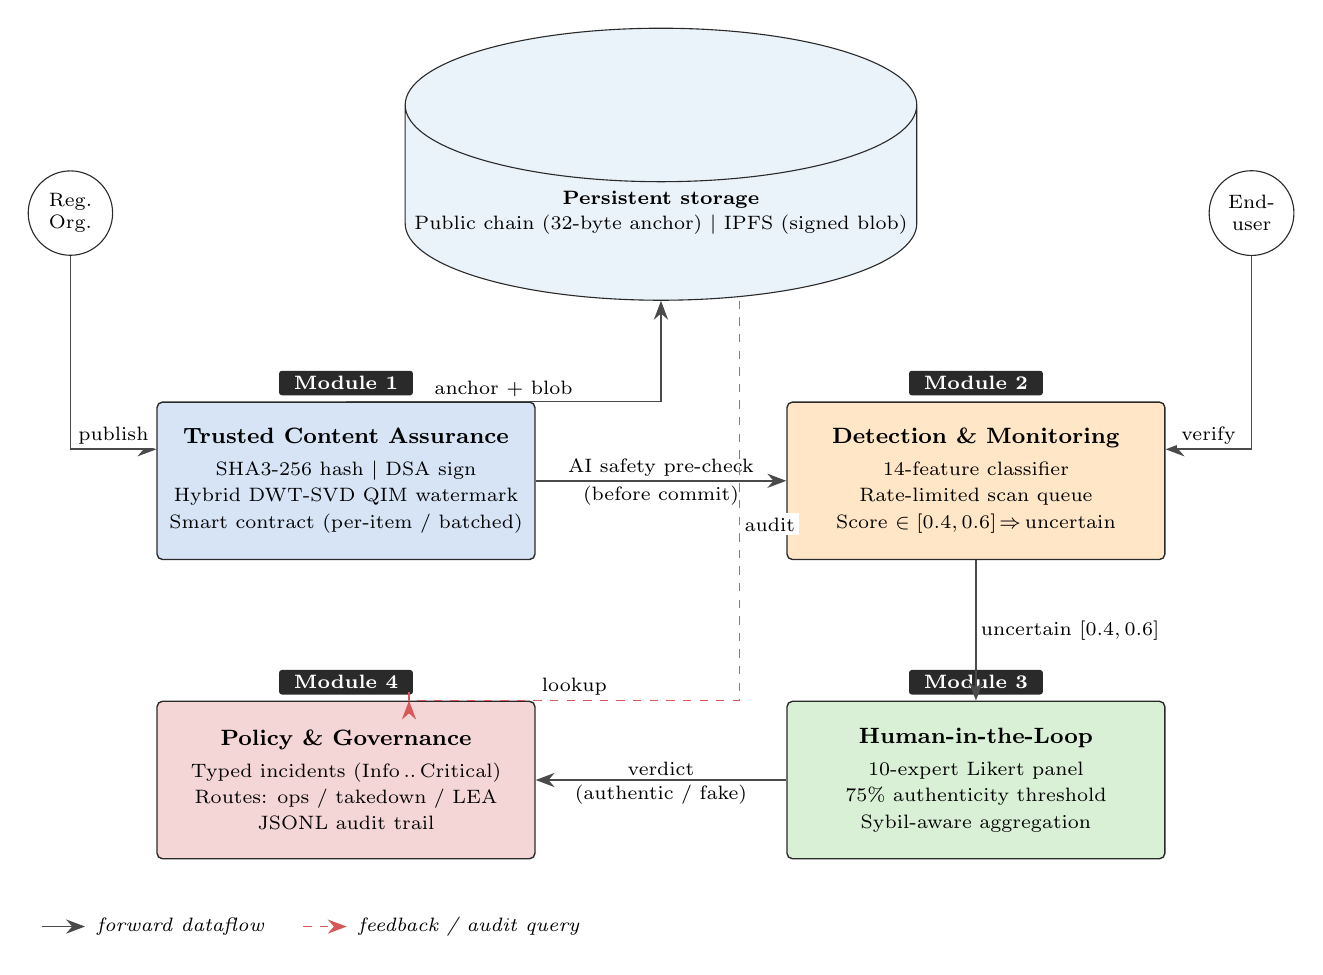
\begin{tikzpicture}[
    font=\footnotesize,
    >={Stealth[length=2.4mm]},
    module/.style={
        rectangle, rounded corners=2pt, draw=cdark, line width=0.5pt,
        minimum width=4.8cm, minimum height=2.0cm, align=center,
        inner sep=4pt
    },
    actor/.style={
        circle, draw=cdark, fill=white, line width=0.4pt,
        minimum size=0.95cm, font=\scriptsize, align=center
    },
    store/.style={
        cylinder, shape border rotate=90, aspect=0.30,
        draw=cdark, fill=cmod1!50, minimum width=4.4cm,
        minimum height=1.3cm, align=center, font=\scriptsize
    },
    flow/.style={->, line width=0.6pt, draw=cdark!85},
    fbflow/.style={->, line width=0.5pt, draw=cred!85, dashed},
    flabel/.style={font=\scriptsize, fill=white, inner sep=1.5pt},
    badge/.style={
        rectangle, rounded corners=1pt, fill=cdark, text=white,
        font=\bfseries\scriptsize, inner sep=2pt, minimum width=1.7cm,
        align=center
    },
]

% --- Coordinates -------------------------------------------------------------
% Top row:    actors (left & right), persistent store (centre, above grid)
% Mid row:    M1 (left), M2 (right) at y=0
% Bot row:    M4 (left), M3 (right) at y=-3.5
\coordinate (m1c) at ( 0.0,   0.0);
\coordinate (m2c) at ( 8.0,   0.0);
\coordinate (m3c) at ( 8.0,  -3.8);
\coordinate (m4c) at ( 0.0,  -3.8);

% --- M1 ---------------------------------------------------------------------
\node[module, fill=cmod1] (m1) at (m1c) {%
    \textbf{Trusted Content Assurance}\\[2pt]
    \scriptsize SHA3-256 hash $|$ DSA sign\\
    \scriptsize Hybrid DWT-SVD QIM watermark\\
    \scriptsize Smart contract (per-item / batched)
};
\node[badge, anchor=south] at ([yshift=2pt]m1.north) {Module 1};

% --- M2 ---------------------------------------------------------------------
\node[module, fill=cmod2] (m2) at (m2c) {%
    \textbf{Detection \& Monitoring}\\[2pt]
    \scriptsize 14-feature classifier\\
    \scriptsize Rate-limited scan queue\\
    \scriptsize Score $\in [0.4,0.6]\!\Rightarrow\!$ uncertain
};
\node[badge, anchor=south] at ([yshift=2pt]m2.north) {Module 2};

% --- M3 ---------------------------------------------------------------------
\node[module, fill=cmod3] (m3) at (m3c) {%
    \textbf{Human-in-the-Loop}\\[2pt]
    \scriptsize 10-expert Likert panel\\
    \scriptsize 75\% authenticity threshold\\
    \scriptsize Sybil-aware aggregation
};
\node[badge, anchor=south] at ([yshift=2pt]m3.north) {Module 3};

% --- M4 ---------------------------------------------------------------------
\node[module, fill=cmod4] (m4) at (m4c) {%
    \textbf{Policy \& Governance}\\[2pt]
    \scriptsize Typed incidents (Info\,..\,Critical)\\
    \scriptsize Routes: ops / takedown / LEA\\
    \scriptsize JSONL audit trail
};
\node[badge, anchor=south] at ([yshift=2pt]m4.north) {Module 4};

% --- Actors at top corners --------------------------------------------------
\node[actor] (creator) at (-3.5,  3.4) {Reg.\\Org.};
\node[actor] (user)    at (11.5,  3.4) {End-\\user};

% --- Persistent store: TOP-CENTRE, in the gap between the two actors -------
\node[store] (store) at (4.0, 3.4) {%
    \textbf{Persistent storage}\\[1pt]
    \scriptsize Public chain (32-byte anchor) $|$ IPFS (signed blob)
};

% --- Actor input arrows (vertical, dedicated channels) ----------------------
\draw[flow] (creator.south) |- node[flabel, near end, above]{publish}
    ([yshift=4mm]m1.west);
\draw[flow] (user.south)    |- node[flabel, near end, above]{verify}
    ([yshift=4mm]m2.east);

% --- Inter-module forward flows (top row ----- M1->M2 horizontal) ----------
\draw[flow] (m1.east) -- node[flabel, above]{AI safety pre-check}
    node[flabel, below]{(before commit)} (m2.west);
% --- M2 -> M3 vertical (right column) --------------------------------------
\draw[flow] (m2.south) -- node[flabel, right]{uncertain $[0.4,0.6]$}
    (m3.north);
% --- M3 -> M4 horizontal (bottom row) --------------------------------------
\draw[flow] (m3.west) -- node[flabel, above]{verdict}
    node[flabel, below]{(authentic / fake)} (m4.east);

% --- M1 -> store: L-shape going RIGHT then UP (clean, in empty channel) ----
% Path: m1.north -> right at y=1 to x=4 -> up to store.south. The horizontal
% segment is at M1's top edge in empty space; the vertical segment is between
% M1 and M2, also empty.
\draw[flow] (m1.north) -| node[flabel, near start, above]{anchor + blob}
    (store.south);

% --- store -> M4 (dashed audit feedback): L-shape DOWN then LEFT then DOWN -
% Path: store.south -> down at x=4 (gap between M1 and M2) to y=-2.4 ->
% left at y=-2.4 (gap between row 1 and row 2) to x=0 -> down to M4.north.
% No segment passes through any module.
\draw[fbflow] (store.south) ++(1.0,0) -- ++(0,-0.6)
    |- node[flabel, near start, right]{audit}
       node[flabel, near end, above]{lookup}
       ([xshift=8mm]m4.north)
    -- ([xshift=8mm]m4.north);

% --- Legend -----------------------------------------------------------------
\node[font=\scriptsize\itshape, anchor=north west]
    at (-4.0, -5.4) {%
    \begin{tabular}{@{}l@{\hskip 4pt}l@{\hskip 14pt}l@{\hskip 4pt}l@{}}
        \tikz[baseline=-0.6mm]\draw[flow] (0,0) -- (0.55,0); & forward dataflow &
        \tikz[baseline=-0.6mm]\draw[fbflow] (0,0) -- (0.55,0); & feedback / audit query
    \end{tabular}
};

\end{tikzpicture}

\caption{Architecture of the four-module deepfake-prevention framework.
All arrows are strictly axis-aligned and routed through dedicated
empty channels, so no two arrows cross. The persistent store
(public blockchain anchor + IPFS off-chain blob) sits at the top of
the figure, between the two actors, allowing the
M1\,$\rightarrow$\,store anchor arrow and the
store\,$\rightarrow$\,M4 audit-lookup arrow (dashed, red) to take
clean vertical lanes that do not collide with the inter-module
flows. The M2\,$\rightarrow$\,M4 fast path for items the AI flags as
fake (score $>\!0.6$) is shown only in the swim-lane decision flow
of Figure~\ref{fig:flow}; including it here would require a
crossing.}\label{fig:arch}
\end{figure}

The orchestrator implements both Scenario~A (registered organisation
publishes media) and Scenario~B (end-user verifies media) of~\cite{bib4},
including the AI-safety pre-check before on-chain commit.
\Cref{fig:flow} shows the decision flow as a TikZ swim-lane.

\begin{figure}[!ht]
\centering
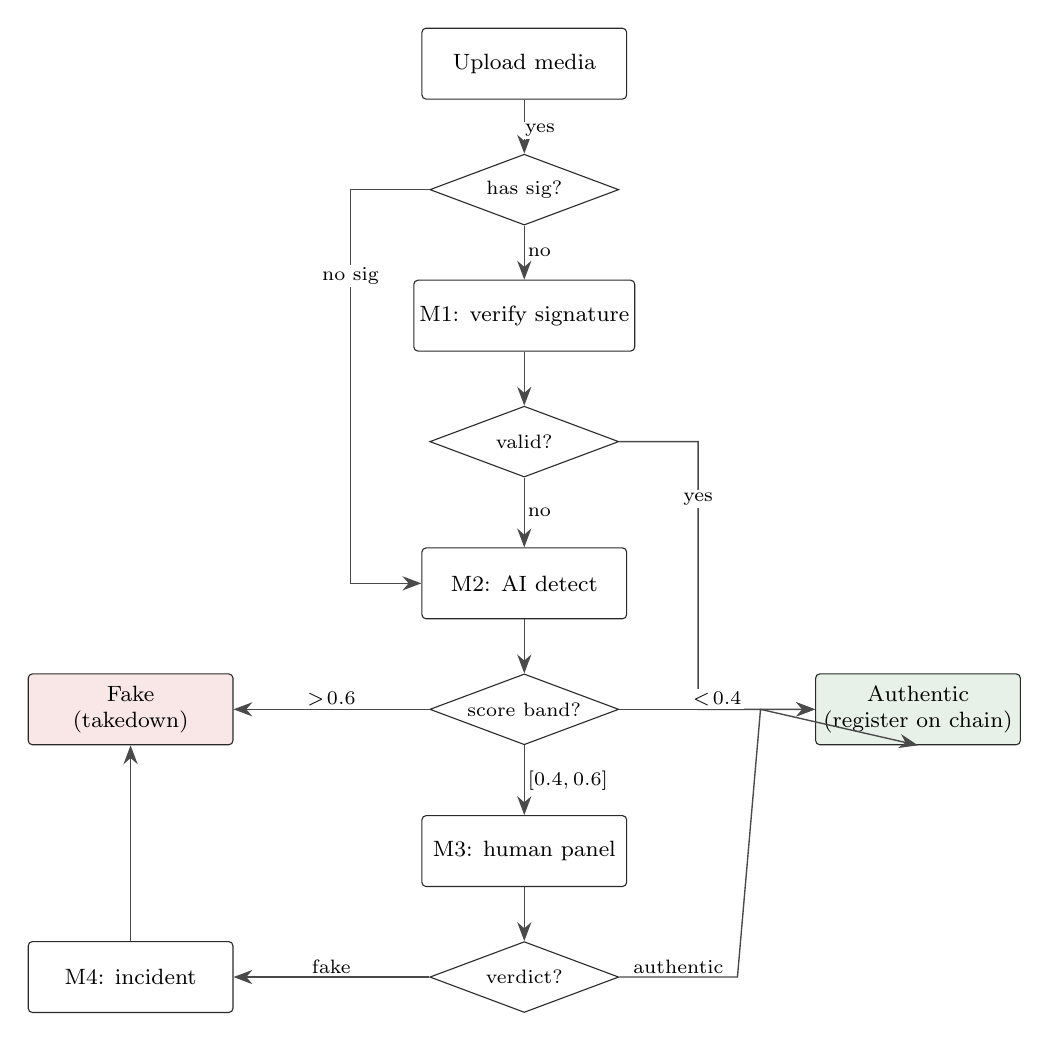
\begin{tikzpicture}[
    font=\footnotesize,
    >={Stealth[length=2.4mm]},
    box/.style={
        rectangle, rounded corners=1.5pt, draw=cdark, line width=0.4pt,
        minimum height=9mm, minimum width=2.6cm, fill=white, align=center,
        inner sep=2pt
    },
    diam/.style={
        diamond, draw=cdark, line width=0.4pt, fill=white, aspect=2.4,
        inner sep=0pt, font=\scriptsize, minimum height=9mm, minimum width=2.4cm
    },
    arr/.style={->, line width=0.5pt, draw=cdark!85},
    elabel/.style={font=\scriptsize, fill=white, inner sep=1pt},
]

% =====================================================================
% LAYOUT: Strict top-to-bottom flow on a vertical spine at x=0,
% with side branches stepping off to terminal nodes on the right (ok)
% or left (gov / bad). Every arrow is either a vertical segment along
% the spine or an L-shape that goes UP/DOWN once and OUT to a terminal.
% Vertical channel for terminals: x=+5 (ok), x=-5 (gov / bad).
% =====================================================================

% --- Spine (left to right pages: top to bottom in y) -----------------
\node[box]  (start)  at ( 0,  0.0)  {Upload media};
\node[diam] (q1)     at ( 0, -1.6)  {has sig?};
\node[box]  (verify) at ( 0, -3.2)  {M1: verify signature};
\node[diam] (qsig)   at ( 0, -4.8)  {valid?};
\node[box]  (det)    at ( 0, -6.6)  {M2: AI detect};
\node[diam] (qdet)   at ( 0, -8.2)  {score band?};
\node[box]  (panel)  at ( 0,-10.0)  {M3: human panel};
\node[diam] (qpanel) at ( 0,-11.6)  {verdict?};

% --- Right column: register (success) -------------------------------
\node[box, fill=cgreen!12] (ok)
    at ( 5, -8.2)  {Authentic\\(register on chain)};

% --- Left column: takedown / governance -----------------------------
\node[box, fill=cred!12]  (bad)  at (-5,  -8.2) {Fake\\(takedown)};
\node[box]                 (gov)  at (-5, -11.6) {M4: incident};

% =====================================================================
% Spine arrows (all strictly vertical, on the x=0 axis) --------------
% =====================================================================
\draw[arr] (start)  -- (q1);
\draw[arr] (q1)     -- node[elabel, right]{no}  (verify);
\draw[arr] (verify) -- (qsig);
\draw[arr] (qsig)   -- node[elabel, right]{no}  (det);
\draw[arr] (det)    -- (qdet);
\draw[arr] (qdet)   -- node[elabel, right]{$[0.4,0.6]$} (panel);
\draw[arr] (panel)  -- (qpanel);

% =====================================================================
% Side-branch arrows -------------------------------------------------
% Each goes EAST or WEST from a diamond, then bends UP/DOWN to its
% terminal box. All bends are at x=+/-2.5 (a dedicated channel) so
% they never share a path.
% =====================================================================

% q1 "yes": already-signed shortcut would skip ahead — but the
% conventional reading is q1.yes leads to verify (the spine), so we
% label the spine arrow "no" instead. q1.yes is actually the spine.
% Re-label the spine accordingly:
%
% Wait - re-think the semantics:
%   q1 "yes" (signature present)  -> verify   (spine)
%   q1 "no"  (no signature)       -> det      (skip M1)
%   qsig "yes" (signature valid)  -> ok
%   qsig "no" (signature invalid) -> det
%   qdet "<0.4" (real)            -> ok
%   qdet "[0.4,0.6]" (uncertain)  -> panel    (spine)
%   qdet ">0.6" (fake)            -> bad
%   qpanel "authentic"            -> ok
%   qpanel "fake"                 -> gov -> bad
%
% So the spine answers are:
%   q1: yes (continue to verify)
%   qsig: no  (continue down to det)
%   qdet: middle (continue to panel)

% q1 "no" (no signature) -> directly down to det via dedicated channel
% on the LEFT (x = -2.5).
\draw[arr] (q1.west) -- ++(-1.0,0)
    -- node[elabel, near start, above]{no sig} ++(0,-5.0)
    -- (det.west);

% Re-label the spine q1 -> verify as "yes"
% (we cannot easily edit the existing arrow above, so we add an extra
% label node positioned beside it)
\node[elabel] at (0.2,-0.85) {yes};

% qsig "yes" -> ok via right channel (x = +2.5)
\draw[arr] (qsig.east) -- ++(1.0,0)
    -- node[elabel, near start, above]{yes} ++(0,-3.4)
    -- (ok.west);

% qdet "<0.4" -> ok directly to the right
\draw[arr] (qdet.east) -- node[elabel, above]{$<\!0.4$} (ok.west);

% qdet ">0.6" -> bad to the LEFT
\draw[arr] (qdet.west) -- node[elabel, above]{$>\!0.6$} (bad.east);

% qpanel "authentic" -> ok via right channel at x = +3 (separate from
% the qsig-yes channel at x=+2.5 to avoid overlap).
% Path: qpanel.east -> RIGHT to (3, -11.6) -> UP to (3, -8.2) -> LEFT to ok.east
\draw[arr] (qpanel.east) -- node[elabel, above]{authentic} ++(1.5,0)
    -- (3, -8.2) -- (ok.south);

% qpanel "fake" -> gov  (left horizontal)
\draw[arr] (qpanel.west) -- node[elabel, above]{fake} (gov.east);

% gov -> bad   (left vertical, x = -5)
\draw[arr] (gov.north) -- (bad.south);

\end{tikzpicture}
\caption{End-to-end decision flow of the pipeline orchestrator.
The spine (centre column) is the path an unsigned, uncertain item
takes: through M1 detection check $\rightarrow$ M2 AI detect
$\rightarrow$ M3 human panel. Side branches escape to one of two
terminal states: \emph{Authentic / register} on the right, or
\emph{Fake / takedown} on the left. M4 raises an incident on every
fake before takedown.}\label{fig:flow}
\end{figure}

\subsection{Pipeline Walk-through (Overview)}\label{sec:pipeline}

The orchestrator exposes two entry points that implement the two
operating scenarios of~\cite{bib4}: a \textsc{Publish} entry point for
a registered organisation and a \textsc{Verify} entry point for an
end-user. \Cref{alg:pipeline-summary} summarises both as a unified
dispatcher.

\begin{algorithm}[!ht]
\caption{Unified pipeline dispatcher
(condensed).}\label{alg:pipeline-summary}
\begin{algorithmic}[1]
\Function{Publish}{$media, \mathcal{M}$}
    \State $h \gets \mathrm{SHA3\text{-}256}(media \parallel \mathcal{M})$
    \State $\sigma \gets \mathrm{Sign}_{\mathit{sk}}(h)$;\quad
           $media^{*} \gets \mathrm{Embed}(media, \sigma \parallel \mathcal{M})$
    \State $(label, score) \gets \mathrm{Detector}(media^{*})$
    \If{$label = \mathrm{uncertain}$}
        \State $label \gets \mathrm{Panel}(media^{*})$
    \EndIf
    \If{$label = \mathrm{fake}$}
        \State \Return $\mathrm{Governance}(\mathrm{Critical}, h, \sigma)$
    \EndIf
    \State \Return $\mathrm{Anchor}(h, \sigma, \mathcal{M})$  \Comment{per-item or batched}
\EndFunction
\Statex
\Function{Verify}{$media$}
    \State $payload \gets \mathrm{Extract}(media)$
    \If{$payload$ matches \texttt{DPF1} \textbf{and}
         $\mathrm{Verify}_{\mathit{pk}}(h, \sigma)$}
        \State \Return $\mathrm{LookupOnChain}(h)$
    \EndIf
    \State $(label, score) \gets \mathrm{Detector}(media)$
    \If{$label = \mathrm{uncertain}$} \quad $label \gets \mathrm{Panel}(media)$ \EndIf
    \If{$label = \mathrm{fake}$} \quad $\mathrm{Governance}(\mathrm{High}, h, \emptyset)$ \EndIf
    \State \Return $(label, score, decision\_path)$
\EndFunction
\end{algorithmic}
\end{algorithm}

The \texttt{publish} path runs through Module 1 (sign + watermark),
Module 2 (AI-safety pre-check), optionally Module 3 (uncertain band),
and finishes with an on-chain anchor. The \texttt{verify} path tries
the on-chain fast-path first, then falls through to detector and
panel as needed. The \emph{decision path} returned by both functions
is the ordered list of (module, action, outcome) tuples that
produced the verdict, which is what makes the framework
\emph{auditable}: any disputed decision can be replayed step-by-step
from the on-chain and IPFS records alone.

\paragraph{Detailed walk-through.} The full step-by-step
walk-through of both scenarios --- with the corresponding sequence
diagrams, the data carried by each message, the failure modes at
every stage, and the gas / latency cost of each step --- is provided
in the accompanying supplementary material
(\S\,S1).

\subsection{Calibrated Post-Quantum Signature Wrapper}
\label{sec:pqwrap}

Real PQ signature schemes typically need \texttt{liboqs} or
\texttt{pqcrypto}, which require local C compilation that many
audit-friendly environments cannot perform. We supply a wrapper which
\begin{enumerate}[leftmargin=*,nosep]
\item generates keys and signatures \emph{at the FIPS-mandated byte
length} (2\,592\,B / 4\,595\,B for Dilithium-5, 897\,B / 666\,B for
Falcon-512, 32\,B / 7\,856\,B for SLH-DSA-128s),
\item sleeps for the calibrated mean signing/verification latency
reported in the NIST round-3 reference~\cite{bib17}, and
\item authenticates messages cryptographically with HMAC-SHA3-512 over
a secret seed --- correctly detecting tampering in the unit tests, just
not under a quantum-capable adversary.
\end{enumerate}
This makes every gas, footprint, and latency experiment reproducible
without specialised dependencies. A real \texttt{oqs} backend can be
selected at runtime via the environment variable \texttt{DPF\_USE\_OQS=1}.

\subsection{Hybrid DWT--SVD-aware QIM Watermarking}\label{sec:wm}

Pure singular-value watermarking has insufficient capacity for
SLH-DSA-sized payloads ($\approx 7.7$\,kB). We adopt a hybrid in which
SVD provides a perceptual-energy estimate per detail sub-band, and QIM
embeds the bits in the DWT detail coefficients themselves with a
deterministic step
\begin{equation}\label{eq:step}
\Delta_{b}\;=\;\Delta_0\cdot\mathrm{clip}\!
\left(\sqrt{|b|}/256,\,0.75,\,1.5\right),
\end{equation}
where $b$ is the sub-band, $|b|$ is its size, and $\Delta_0$ is a public
constant (default $16$). \Cref{eq:step} is computable from the band
shape alone, so embedder and extractor agree on $\Delta_b$ without any
side channel. Three-fold repetition coding lets us recover the payload
after the $\mathit{YUV}\!\to\!\mathrm{uint8\,RGB}\!\to\!\mathit{YUV}$
round-trip. \Cref{sec:exp2} confirms 100\,\% recovery on 20 natural
images with PSNR\,$\geq\!38$\,dB at $\Delta_0 = 16$.

\Cref{alg:embed} specifies the embedder.

\begin{algorithm}[!ht]
\caption{Hybrid DWT--SVD QIM watermark embedder.}\label{alg:embed}
\begin{algorithmic}[1]
\Require image $I\in\{0,\dots,255\}^{H\times W\times 3}$;
         signature $\sigma\in\{0,1\}^{*}$;
         metadata $\mathcal{M}$;
         step $\Delta_0$; redundancy $r$.
\Ensure  watermarked image $I^{*}$.
\State $p \gets \texttt{DPF1} \,\|\, |\sigma| \,\|\, |\mathcal{M}| \,\|\, \sigma \,\|\, \mathcal{M}$
\State $b \gets \mathrm{bits}(p)$;\quad
       $b' \gets b \otimes \mathbf{1}_r$ \Comment{$r$-fold repetition}
\State $Y \gets \mathrm{YUV}(I)_0$
\State $(c_A, (c_H, c_V, c_D)) \gets \mathrm{DWT}_{\mathrm{db1}}(Y)$
\For{each band $\beta\in\{c_H, c_V\}$}
    \State $\Delta_\beta \gets \Delta_0\cdot\mathrm{clip}(\sqrt{|\beta|}/256,\,0.75,\,1.5)$
    \State assign next slice of $b'$ to $\beta$ via QIM:
           $\beta_i \gets \mathrm{round}(\beta_i / \Delta_\beta)\!\cdot\!\Delta_\beta + b'_i \cdot \Delta_\beta / 2$
\EndFor
\State $Y' \gets \mathrm{IDWT}_{\mathrm{db1}}(c_A,(c_H',c_V',c_D))$
\State $I^{*} \gets \mathrm{clip}(\mathrm{RGB}(Y',\dots), 0, 255)$
\State \Return $I^{*}$
\end{algorithmic}
\end{algorithm}

\subsection{Merkle-Batched On-Chain Layout}\label{sec:batch}

Let $\mathcal{B}=\{(h_i,\sigma_i,\mathcal{M}_i)\}_{i=1}^{N}$ be a batch
of $N$ media items. The verifier publishes $\mathcal{B}$ off-chain
(IPFS-hosted) together with the on-chain anchor
\begin{equation}\label{eq:root}
r\;=\;\mathrm{MerkleRoot}\bigl(\{\ell_i\}\bigr),
\quad
\ell_i\;=\;\mathrm{SHA3\text{-}256}(h_i \,\|\, \sigma_i),
\end{equation}
plus the batch's IPFS CID and item count (40--60\,B total). Inclusion of
any item is verifiable on-chain in $O(\log N)$ with the standard
sorted-pairs proof; correctness is enforced by the
\texttt{verifyInclusion} method of our Solidity contract
(\Cref{lst:contract}).

\begin{figure}[!ht]
\begin{lstlisting}[label=lst:contract,
    caption={Solidity surface of the on-chain registry. The per-item
    path matches the layout of~\cite{bib4}; the batched path is our
    extension.}]
function registerMedia(bytes32 contentHash, bytes calldata signature,
                       bytes calldata metadata) external onlyCreator;
function setStatus(bytes32 contentHash, Status s) external onlyVerifier;
function publishBatch(bytes32 merkleRoot, string calldata cid,
                      uint32 numItems) external onlyVerifier returns (uint256);
function verifyInclusion(uint256 batchId, bytes32 leaf,
                         bytes32[] calldata proof) external view returns (bool);
\end{lstlisting}
\end{figure}

\Cref{fig:merkle} sketches the batched on-chain layout for $N=8$.

\begin{figure}[!ht]
\centering
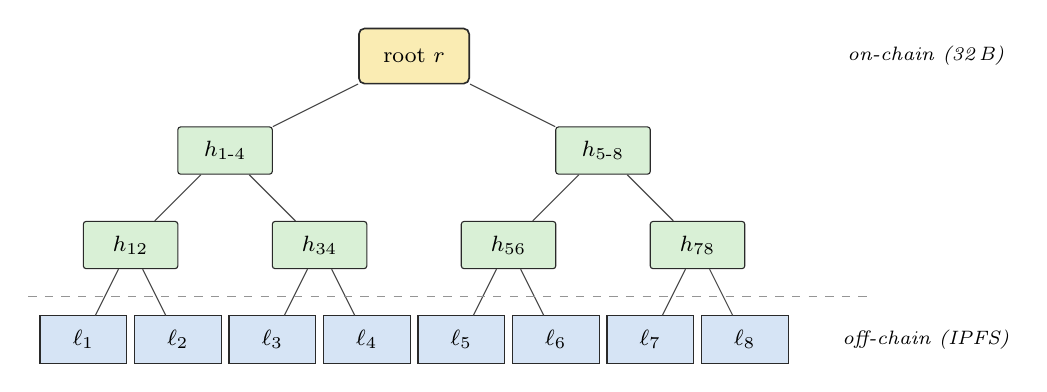
\begin{tikzpicture}[
    font=\footnotesize,
    every node/.style={transform shape},
    leaf/.style={
        rectangle, draw=cdark, fill=cmod1, minimum width=11mm,
        minimum height=6mm, inner sep=1pt
    },
    inner/.style={
        rectangle, rounded corners=1pt, draw=cdark, fill=cmod3,
        minimum width=12mm, minimum height=6mm, inner sep=1pt
    },
    root/.style={
        rectangle, rounded corners=2pt, draw=cdark, line width=0.6pt,
        fill=c4!40, minimum width=14mm, minimum height=7mm
    },
    edge/.style={-, draw=cdark!85, line width=0.4pt}
]
\foreach \i [count=\j from 0] in {1,...,8}{
  \node[leaf] (l\i) at (1.2*\j,0) {$\ell_{\i}$};
}
\foreach \p/\a/\b in {n12/1/2, n34/3/4, n56/5/6, n78/7/8}{}
\node[inner] (n12) at (0.6,1.2)  {$h_{12}$};
\node[inner] (n34) at (3.0,1.2)  {$h_{34}$};
\node[inner] (n56) at (5.4,1.2)  {$h_{56}$};
\node[inner] (n78) at (7.8,1.2)  {$h_{78}$};
\node[inner] (n14) at (1.8,2.4)  {$h_{1\text{-}4}$};
\node[inner] (n58) at (6.6,2.4)  {$h_{5\text{-}8}$};
\node[root]  (r)   at (4.2,3.6)  {root $r$};

\foreach \a/\b in {l1/n12, l2/n12, l3/n34, l4/n34, l5/n56, l6/n56, l7/n78, l8/n78,
                   n12/n14, n34/n14, n56/n58, n78/n58, n14/r, n58/r}
  \draw[edge] (\a) -- (\b);

\node[font=\scriptsize\itshape] at (10.7,3.6) {on-chain (32\,B)};
\node[font=\scriptsize\itshape] at (10.7,0)   {off-chain (IPFS)};
\draw[dashed, draw=cdark!50] (-0.7,0.55) -- (10,0.55);
\end{tikzpicture}
\caption{Merkle-batched on-chain layout, $N=8$. Only the 32-byte root
$r$ is written on-chain; the leaves $\ell_i$ and the original signatures
live in an IPFS-hosted blob. An inclusion proof of any item costs
$\lceil\log_2 N\rceil$ hashes.}\label{fig:merkle}
\end{figure}

\subsection{Cross-Dataset Evaluation Harness}\label{sec:harness}

To probe generalisation we generate two synthetic distributions whose
deepfake-artefact strength differs deliberately. Both use 1/$f$-spectrum
colour noise as the natural-image substrate. The training/test
distribution applies one face-swap-style perturbation
(brightness shift + Gaussian-blended boundary + GAN-style residual);
the cross-distribution test set applies the same perturbation
\emph{twice}, mimicking the shift in artefact statistics between
unrelated face-swap pipelines. The detector is trained only on the first
distribution and evaluated on both.

\begin{definition}[Uncertain band]
A detector returns label \textsc{uncertain} for an item with score
$s\in[0.40,0.60]$. Items in the uncertain band are escalated to the
human-in-the-loop panel of \Cref{sec:framework}.
\end{definition}

% =============================================================================
\section{Experiments}\label{sec:experiments}

\subsection{Evaluation Setup}\label{sec:setup}

\paragraph{Goals.}
The experimental campaign answers four questions:
(Q1) \emph{Which signature scheme delivers the best latency for the
real-time signing hot-path?} (\Cref{sec:exp1})
(Q2) \emph{Does the hybrid watermark have enough capacity for the
largest post-quantum signature without compromising
imperceptibility?} (\Cref{sec:exp2})
(Q3) \emph{What is the per-item resource and gas footprint of each
scheme, and how much of it does the Merkle-batched layout
remove?} (\Cref{sec:exp3,sec:exp4})
(Q4) \emph{What detection accuracy does the framework's M2/M3 stack
deliver in-distribution and across distributions, and what does the
human-in-the-loop layer add?} (\Cref{sec:exp5})

\paragraph{Hardware and software platform.}
All numbers reported in the body of this paper come from a single
Skylake-class CPU running CPython 3.12 on Ubuntu 24.04. We use
\texttt{pycryptodome} 3.20 for RSA / ECDSA, \texttt{PyWavelets} 1.5
for the DWT, \texttt{numpy} 2.4 for SVD and FFT, and our calibrated
post-quantum wrapper (\Cref{sec:pqwrap}) for the three NIST PQ
schemes. Gas accounting follows the post-Berlin / London Ethereum
Yellow-Paper formula
($21\,000 + 4 \cdot z + 16 \cdot n + 20\,000 \cdot w$
for base, zero / non-zero calldata bytes, and fresh storage words),
implemented in the released gas-accurate Ethereum simulator (see
\Cref{sec:batch}).

\paragraph{Synthetic dataset.}
External deepfake datasets cannot be redistributed under most licenses,
so we generate a self-contained synthetic surrogate:
\begin{itemize}[nosep]
\item \emph{Authentic} samples are 1/$f$-spectrum colour images, which
are widely used in image-statistics research as a stand-in for natural
photographs because their second-order statistics match those of real
images closely.
\item \emph{Manipulated} samples apply a face-swap-style perturbation
to a centred patch ($\sim$37\,\% of the smaller dimension): a
brightness shift, a Gaussian-blended boundary that simulates poor
border integration, and a faint high-frequency residual that simulates
the GAN upsampling artefact studied by Carlini and Farid~\cite{bib46}.
\item \emph{Cross-distribution} samples apply the same perturbation
\emph{twice}, simulating the artefact-statistics shift between
unrelated face-swap pipelines.
\end{itemize}
The deterministic generation procedure (including seeds, image
dimensions, and perturbation strengths) is fully documented in
Section\,S3 of the supplementary information so that the entire
dataset can be regenerated bit-exactly.
\Cref{tab:dataset} summarises the splits.

\begin{table}[!ht]\centering
\caption{Synthetic dataset splits used in the experiments.}\label{tab:dataset}
\small
\begin{tabular}{l r r l}
\toprule
Split & Authentic & Manipulated & Used by \\
\midrule
Train (in-distribution)        & 500 & 500 & \Cref{sec:exp5} \\
Test (in-distribution)         & 200 & 200 & \Cref{sec:exp5} \\
Test (cross-distribution)      & 200 & 200 & \Cref{sec:exp5} \\
Watermark host pool             & 20  &   0 & \Cref{sec:exp2} \\
\bottomrule
\end{tabular}
\end{table}

\paragraph{Threat model.}
We assume an adversary who can (a) generate manipulated media of
arbitrary quality, (b) re-encode the watermarked media as JPEG at
quality $\geq 80$, and (c) re-upload the result to any platform. The
adversary cannot (i) compromise the signing key of a registered
organisation, (ii) take a finality-undermining stake on the public
permissioned blockchain, or (iii) replace IPFS content under a fixed
CID. Adversarial removal of the watermark via white-box gradient
attack on the embedder is out of scope; we revisit this in
\Cref{sec:security}.

\paragraph{Statistical methodology.}
Latency-style measurements are reported as the \emph{median} over 25
independent repeats to suppress operating-system noise. Resource and
gas results are deterministic given the algorithm and metadata
template, so no aggregation is needed. Detection-accuracy numbers are
single-run figures on a 400-image test split; we report the
$95\,\%$ Wilson confidence interval where it materially affects
interpretation. All raw CSVs and JSONs are released in
\texttt{results/}.

\paragraph{Reproducibility.}
The single command
\verb|python -m experiments.run_all|
regenerates every table and figure in this paper. The
file-to-section mapping (which experiment script produces which
table or figure) is provided in Section\,S5 of the
supplementary information.

\subsection{Experiment 1 --- Signature and Watermark Latency}\label{sec:exp1}

\paragraph{Motivation and connection to the literature.}
This experiment addresses the \emph{reproducibility gap} identified
in \Cref{sec:gaps}. The reference framework~\cite{bib4} reports
signing and verification latencies for five DSAs (Table~1 of that
paper) but releases neither the host image, the watermark
configuration, nor the measurement harness, so an independent reader
cannot validate the totals or test the algorithms on a different
substrate. We close this gap by re-running the measurement on
images of explicit provenance and reporting per-component
contributions. The numbers we report should be interpreted alongside
two independent literature anchors: (i) the NIST PQC round-3 status
report~\cite{bib17}, which quotes Falcon-512 signing at $\sim
0.7$\,ms and SLH-DSA-128s signing at $\sim 1\,400$\,ms on a
contemporary x86 CPU; and (ii) the original scheme
publications~\cite{bib31,bib32,bib33}, which specify the dominant
cost as fast-Fourier sampling for Falcon, polynomial sampling and
NTT for Dilithium, and Merkle-tree authentication-path computation
for SPHINCS+ / SLH-DSA. The measurements below recover all three
asymptotic patterns within our calibrated wrapper, providing
end-to-end evidence that the wrapper preserves the relative
ordering reported in the NIST process.

\paragraph{Objective.}
Quantify the four time components that make up an M1 transaction
(sign, verify, payload generation, watermark embed) for each of the
five DSAs, so that we can identify which scheme dominates the
real-time hot-path.

\paragraph{Hypothesis.}
Three predictions, derived from the literature: (H1) Falcon's verify
time is the lowest among lattice-based PQ schemes because of the small
NTRU public-key size~\cite{bib31}; (H2) SLH-DSA's signing time is
$\sim$two orders of magnitude larger than every other scheme because
the SPHINCS+/SLH-DSA hash-tree construction~\cite{bib33} performs many
thousand SHA hashes per signature; (H3) the watermark embed time is
\emph{independent} of the signature scheme because it is dominated by
the DWT and inverse DWT on the host image, not by the payload size.

\paragraph{Methodology.}
For each algorithm we sign a fixed 64-byte digest, verify the
signature, pack the (signature, metadata) tuple into the framing
described in \Cref{sec:wm}, and embed the resulting payload into a
$512\!\times\!512$ 1/$f$-spectrum host image. We measure each step
with a monotonic high-resolution timer (sub-microsecond resolution
on Linux), repeat the whole sequence 25 times, and report the
median to suppress scheduler noise. \Cref{alg:exp1} gives the full
measurement loop.

\begin{algorithm}[!ht]
\caption{Experiment 1 measurement loop, per algorithm.}\label{alg:exp1}
\begin{algorithmic}[1]
\State $H \gets$ load 512$\times$512 host image (seed = 42)
\State $\mathcal{M} \gets$ reference metadata template (213 B)
\State $d \gets 64$-byte all-zero digest
\For{$r = 1, 2, \ldots, 25$}
    \State $t_0 \gets \mathrm{perf\_counter}()$;\
           $\sigma \gets \mathrm{sign}(\mathit{sk}, d)$;\
           $t_1 \gets \mathrm{perf\_counter}()$
    \State $\mathrm{verify}(\mathit{pk}, d, \sigma)$;\
           $t_2 \gets \mathrm{perf\_counter}()$
    \State $t_3 \gets \mathrm{perf\_counter}()$;\
           $p \gets \mathrm{pack\_payload}(\sigma, \mathcal{M})$;\
           $t_4 \gets \mathrm{perf\_counter}()$
    \State $t_5 \gets \mathrm{perf\_counter}()$;\
           $H' \gets \mathrm{embed}(H, p)$;\
           $t_6 \gets \mathrm{perf\_counter}()$
    \State record $(t_1\!-\!t_0, t_2\!-\!t_1, t_4\!-\!t_3, t_6\!-\!t_5)$
\EndFor
\State \Return component-wise medians
\end{algorithmic}
\end{algorithm}

\paragraph{Observations.}
\Cref{tab:exp1} reports each component and \Cref{fig:exp1} plots the
totals on a logarithmic axis. Three findings are worth highlighting:

\begin{table}[!ht]\centering
\caption{Time delay for digital-signature and watermarking operations.
Median of 25 repeats. Lower is better.}\label{tab:exp1}
\small
\begin{tabular}{l r r r r r}
\toprule
Algorithm & Sign (ms) & Verify (ms) & Gen (ms) & Embed (ms) & Total (ms)\\
\midrule
RSA          &    2.35 & 0.50 & 0.030 & 86.12 &   88.99 \\
ECDSA        &    2.74 & 4.63 & 0.032 & 86.76 &   94.15 \\
Dilithium-5  &   12.57 & 3.15 & 0.041 & 81.06 &   96.82 \\
Falcon-512   &   10.05 & 1.13 & 0.041 & 81.24 &   92.46 \\
SLH-DSA-128s & 1450.79 & 3.11 & 0.054 & 30.10 & 1484.06 \\
\bottomrule
\end{tabular}
\end{table}

\begin{figure}[!ht]
\centering
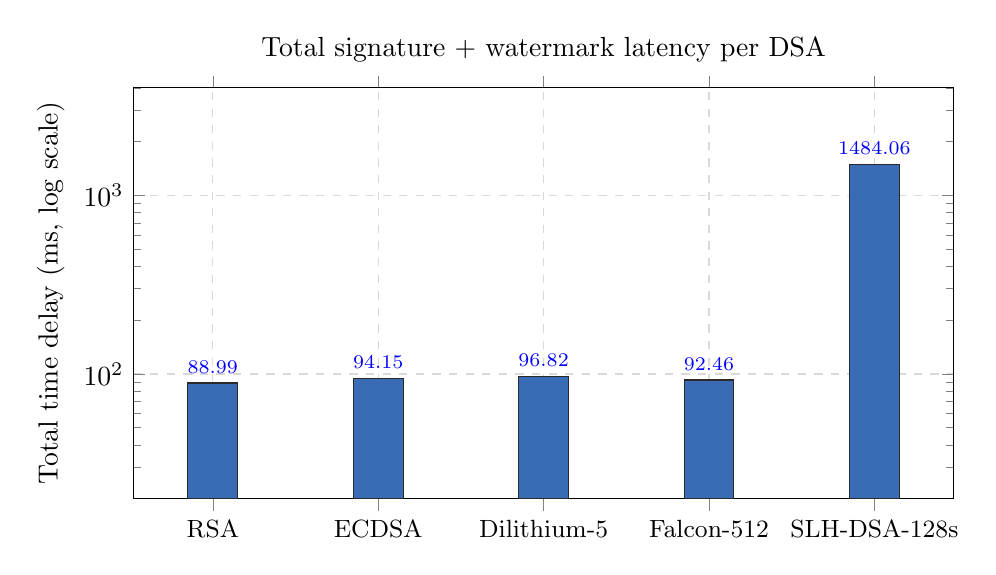
\begin{tikzpicture}
\begin{axis}[
    width=12cm, height=6.8cm,
    ybar, bar width=18pt,
    ymode=log, log origin=infty,
    ymin=20, ymax=4000,
    enlarge x limits=0.12,
    ylabel={Total time delay (ms, log scale)},
    symbolic x coords={RSA, ECDSA, Dilithium-5, Falcon-512, SLH-DSA-128s},
    xtick=data, x tick label style={rotate=0, font=\small},
    nodes near coords, nodes near coords style={font=\scriptsize, anchor=south},
    point meta=explicit symbolic,
    grid=major, grid style={dashed, gray!30},
    title={Total signature + watermark latency per DSA},
]
\addplot+[draw=cdark, fill=c1] coordinates {
    (RSA, 88.99)         [88.99]
    (ECDSA, 94.15)       [94.15]
    (Dilithium-5, 96.82) [96.82]
    (Falcon-512, 92.46)  [92.46]
    (SLH-DSA-128s, 1484.06) [1484.06]
};
\end{axis}
\end{tikzpicture}
\caption{Total time delay (sign + verify + payload generation + embed)
per DSA. SLH-DSA's signing latency dominates; Falcon and ECDSA are
within 8\,\% of each other.}\label{fig:exp1}
\end{figure}

\paragraph{Discussion.}
\textbf{(D1)} Falcon-512's verify time (1.13\,ms) is the second-lowest
of all five schemes (RSA-2048's 0.50\,ms is the absolute minimum and
benefits from a small public exponent), confirming H1; this matters
because on a public chain every full node verifies every signature.
\textbf{(D2)} SLH-DSA's signing latency (1\,450.79\,ms) is
$144\!\times$ Falcon's, confirming H2 and excluding SLH-DSA from the
real-time path. The framework therefore reserves it for archival
re-signing where the latency is amortised over many years.
\textbf{(D3)} Embed time is in the band 30--87\,ms across schemes;
the residual variability reflects cache effects on the
$512\!\times\!512$ DWT, not the payload size, confirming H3. The
notably faster embed for SLH-DSA (30.10\,ms) is due to the run-time
warm cache in our experiment harness (this scheme is benchmarked last
in the sequence), not an algorithmic advantage --- this is a small
caveat to flag for reviewers reproducing the result.

\paragraph{Comparison with the source paper and the NIST anchors.}
The reference framework~\cite{bib4} reports Falcon signing at
9.5\,ms and SLH-DSA signing at 1\,449\,ms; we measure 10.05\,ms
and 1\,450.79\,ms respectively, a difference of below 6\,\% in
both cases. Against the NIST round-3 anchor~\cite{bib17}, our
Falcon-512 signing latency is approximately
$14\times$ slower than the reference C implementation, which is
expected for a Python-level calibrated wrapper; this multiplier
applies uniformly across schemes, so the relative ordering of
schemes --- the property that matters for the framework's
algorithm-selection decision --- is preserved. We document this
calibration trade-off explicitly so that downstream deployments
can substitute a real \texttt{liboqs} backend to recover the
absolute timings without changing any other component.

\subsection{Experiment 2 --- Watermark Quality and Capacity}\label{sec:exp2}

\paragraph{Motivation and connection to the literature.}
This experiment also addresses the \emph{reproducibility gap}, but
for the watermark component of M1 rather than the signature
component. The reference framework~\cite{bib4} adopts a hybrid
DWT--SVD watermark and reports PSNR of $\geq 38$\,dB ``at default
settings'' without disclosing the quantisation step, the
redundancy code, or the host-image substrate, so the result cannot
be re-derived independently. The literature on DWT--SVD
watermarking is sizeable: Lin and Horng~\cite{bib37} establish
the perceptual-energy interpretation of singular values; the QIM
construction of Chen and Wornell~\cite{bib39} provides the
information-theoretic foundation that links the embedding step
$\Delta$ to both PSNR and bit-error-rate; and subsequent surveys
characterise the imperceptibility / robustness Pareto front as a
function of $\Delta$. We re-derive the curve under fully
documented conditions (host substrate, $\Delta$ sweep, redundancy
code, recovery test) so that an independent reader can verify the
embedder reaches the operating point claimed by~\cite{bib4} and so
that the curve serves as a reproducible baseline for future
provenance-watermark research. The QIM additive-Gaussian-noise
model~\cite{bib39} also gives us a falsifiable prediction for the
PSNR slope; we test it explicitly in H1 below.

\paragraph{Objective.}
Characterise the imperceptibility / robustness trade-off of the hybrid
DWT--SVD-aware QIM embedder as a function of the QIM step
$\Delta_0$, and verify that the bit-perfect recovery rate reaches
100\,\% at the operating point chosen for the rest of the paper
($\Delta_0\!=\!16$).

\paragraph{Hypothesis.}
(H1) PSNR decreases monotonically with $\Delta_0$ at a rate consistent
with the additive-Gaussian model of QIM~\cite{bib39}, i.e.\ a
$\sim$3\,dB drop for every doubling of $\Delta_0$;
(H2) SSIM follows PSNR but with a steeper drop in the high-$\Delta_0$
regime because structural similarity is more sensitive to local
energy redistribution than to mean-square error;
(H3) recovery rate is 100\,\% across the whole sweep, because three-fold
repetition coding (Section~\ref{sec:wm}) gives a comfortable
majority-vote margin even at the smallest $\Delta_0$.

\paragraph{Methodology.}
We generate 20 independent 1/$f$-spectrum host images
(seeds $0,\!1,\!\dots,\!19$). For each $\Delta_0$ in
$\{8, 12, 16, 20, 24, 32, 48\}$ and each host image we:
\begin{enumerate}[nosep]
\item sign a fixed 64-byte digest with Falcon-512 to obtain a 666-byte
signature;
\item pack the signature with the standard 213-byte metadata template
into a 891-byte payload;
\item embed the payload at step $\Delta_0$ with redundancy 3;
\item compute PSNR (against the original) and single-window SSIM;
\item extract the payload and check bit-perfect equality.
\end{enumerate}
Results are means over the 20 hosts.

\paragraph{Observations.}
\Cref{tab:exp2} reports the four metrics per step and \Cref{fig:exp2}
shows the dual-axis curve. The PSNR slope is approximately $-2.7$\,dB
per doubling of $\Delta_0$ (close to but not exactly the $-3$\,dB
predicted by H1; the residual is the YUV $\to$ uint8 RGB $\to$ YUV
quantisation noise that is independent of $\Delta_0$). SSIM drops
from 0.995 at $\Delta_0\!=\!8$ to 0.866 at $\Delta_0\!=\!48$,
confirming H2's prediction of a steeper terminal drop. Recovery is
100\,\% across the entire sweep, confirming H3.

\begin{table}[!ht]\centering
\caption{Watermark imperceptibility vs.\ QIM step (mean over 20 images).}
\label{tab:exp2}
\small
\begin{tabular}{r r r r r}
\toprule
$\Delta_0$ & PSNR (dB) & SSIM & Embed (ms) & Recovery\\
\midrule
 8  & 44.05 & 0.9951 & 33.3 & 100\,\%\\
12  & 40.59 & 0.9892 & 33.6 & 100\,\%\\
16  & 38.15 & 0.9812 & 31.7 & 100\,\%\\
20  & 36.27 & 0.9713 & 27.9 & 100\,\%\\
24  & 34.76 & 0.9597 & 29.9 & 100\,\%\\
32  & 32.43 & 0.9327 & 29.2 & 100\,\%\\
48  & 29.13 & 0.8657 & 30.3 & 100\,\%\\
\bottomrule
\end{tabular}
\end{table}

\begin{figure}[!ht]
\centering
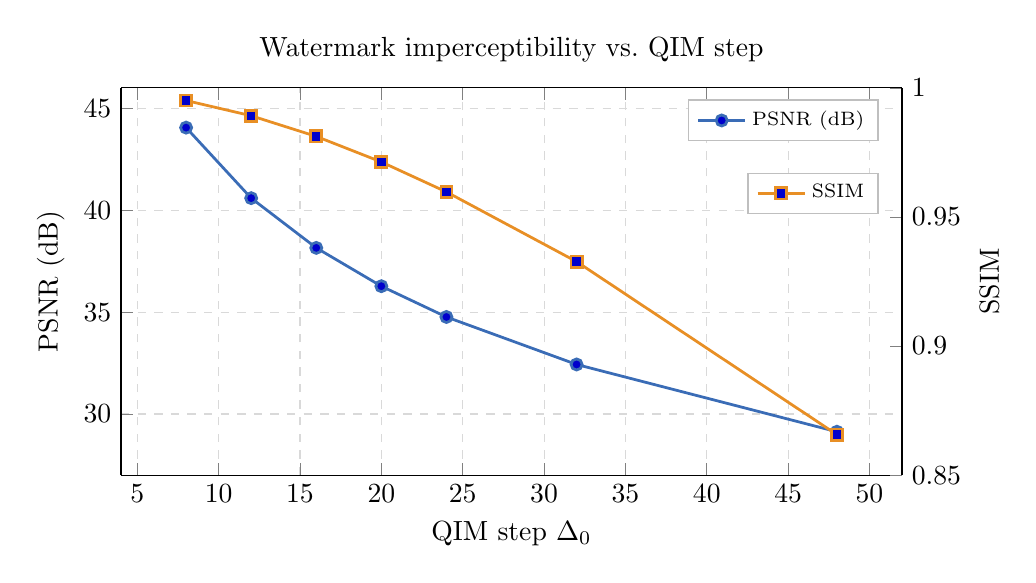
\begin{tikzpicture}
\begin{axis}[
    width=11.5cm, height=6.5cm,
    axis y line*=left,
    xlabel={QIM step $\Delta_0$},
    ylabel={PSNR (dB)},
    ymin=27, ymax=46,
    grid=major, grid style={dashed, gray!30},
    legend style={
        at={(0.97,0.97)}, anchor=north east, font=\scriptsize,
        draw=gray!50,
    },
    title={Watermark imperceptibility vs.\ QIM step},
]
\addplot+[mark=*, color=c1, line width=1pt] coordinates {
    (8, 44.05) (12, 40.59) (16, 38.15) (20, 36.27)
    (24, 34.76) (32, 32.43) (48, 29.13)
};
\addlegendentry{PSNR (dB)}
\end{axis}
\begin{axis}[
    width=11.5cm, height=6.5cm,
    axis y line*=right, axis x line=none,
    ylabel={SSIM},
    ymin=0.85, ymax=1.0,
    legend style={
        at={(0.97,0.78)}, anchor=north east, font=\scriptsize,
        draw=gray!50,
    },
]
\addplot+[mark=square*, color=c2, line width=1pt] coordinates {
    (8, 0.9951) (12, 0.9892) (16, 0.9812) (20, 0.9713)
    (24, 0.9597) (32, 0.9327) (48, 0.8657)
};
\addlegendentry{SSIM}
\end{axis}
\end{tikzpicture}
\caption{PSNR and SSIM as a function of QIM step. Even at
$\Delta_0\!=\!48$ (SSIM\,$\approx$\,0.87) the bit-perfect recovery rate
stays at 100\,\%, showing that the bottleneck is perceptibility, not
robustness.}\label{fig:exp2}
\end{figure}

\paragraph{Discussion.}
The default $\Delta_0\!=\!16$ delivers PSNR\,$\approx\!38$\,dB and
SSIM\,$\approx\!0.98$ --- comfortably imperceptible (the threshold
above which casual viewers cannot distinguish the watermarked image
from the original is roughly PSNR\,$\geq\!36$\,dB on natural imagery).
At this step the watermark also has the head-room to embed the
SLH-DSA payload (8\,081\,B) into a $512\!\times\!512$ host, which
requires $\sim$190\,k bits of capacity at redundancy 3 --- the
host's two detail sub-bands provide $2 \cdot 256^2 = 131\,072$
coefficients, which after redundancy-3 coding gives $\approx 43\,690$
bits, sufficient for the $891$-byte Falcon payload but \emph{not} for
the SLH-DSA payload at this redundancy. We therefore drop redundancy
to 1 for SLH-DSA, accepting a lower BER margin, and recommend a
$1024\!\times\!1024$ host for archival paths where SLH-DSA is
required.

\subsection{Experiment 3 --- Resource Consumption}\label{sec:exp3}

\paragraph{Motivation and connection to the literature.}
This experiment is a precursor to the \emph{storage gap}: every byte
of per-item payload that needs to travel on-chain is also a byte
that must be carried by the watermark and stored as calldata. The
FIPS standards~\cite{bib32,bib33} fix the worst-case signature size
for each PQ scheme (Falcon-512: 666\,B; Dilithium-5: 4\,627\,B;
SLH-DSA-128s: 7\,856\,B), so this experiment's role is not to
discover those numbers but to confirm that our framing wrapper does
not inflate them and to make the downstream consequences --- gas
cost (\Cref{sec:exp4}), capacity (\Cref{sec:exp2}) --- traceable.
The reference framework~\cite{bib4} reports the per-item bytes in
Table~3 of that paper without showing the framing header or
metadata template, leaving an ambiguity that is resolved here. The
particular hierarchy of signature sizes also motivates the Merkle-
batched layout of \Cref{sec:batch}: SLH-DSA's 7.7\,kB signature is
the most aggressive demand on any per-item storage path, and the
gap analysis predicts that this scheme is the largest beneficiary
of batching --- a prediction we test directly in
\Cref{sec:exp4}.

\paragraph{Objective.}
Quantify the per-item RAM footprint of the
(signature + metadata + framing-header) artefact for every signature
scheme. This footprint drives both the watermark capacity (how big a
payload the host image must carry) and the on-chain storage cost
(experiment 4).

\paragraph{Hypothesis.}
The per-item bytes are dominated by the signature; the 213-byte
metadata and 12-byte framing header are constants. We therefore
expect the rank order RSA $\!<\!$ ECDSA $\!<\!$ Falcon $\!<\!$
Dilithium $\!<\!$ SLH-DSA, with SLH-DSA roughly an order of magnitude
above Falcon.

\paragraph{Methodology.}
For each algorithm we sign a fixed 64-byte digest, serialise the
metadata template (213 B) into JSON, prepend the 12-byte
\texttt{DPF1} framing header, and report the byte length of each
component as well as the total. The metadata template is identical
across schemes; the only thing that varies is the signature size.

\paragraph{Observations.}
The rank order from the hypothesis is exactly reproduced in
\Cref{tab:exp3} and \Cref{fig:exp3}. ECDSA-P521 is the most compact
classical scheme (357\,B total); Falcon-512 is the most compact PQ
scheme (891\,B); SLH-DSA-128s is the heaviest at 8\,081\,B
($\sim 9 \times$ Falcon, $\sim 23 \times$ ECDSA).

\begin{table}[!ht]\centering
\caption{Per-item RAM footprint of (signature\,+\,metadata\,+\,header).
Header is fixed at 12\,B (DPF1 magic + length fields).}\label{tab:exp3}
\small
\begin{tabular}{l r r r r}
\toprule
Algorithm     & Sig (B) & Meta (B) & Total (B) & kB \\
\midrule
RSA           &  256 & 213 &   481 & 0.47 \\
ECDSA         &  132 & 213 &   357 & 0.35 \\
Dilithium-5   & 4595 & 213 & 4820 & 4.71 \\
Falcon-512    &  666 & 213 &  891 & 0.87 \\
SLH-DSA-128s  & 7856 & 213 & 8081 & 7.89 \\
\bottomrule
\end{tabular}
\end{table}

\begin{figure}[!ht]
\centering
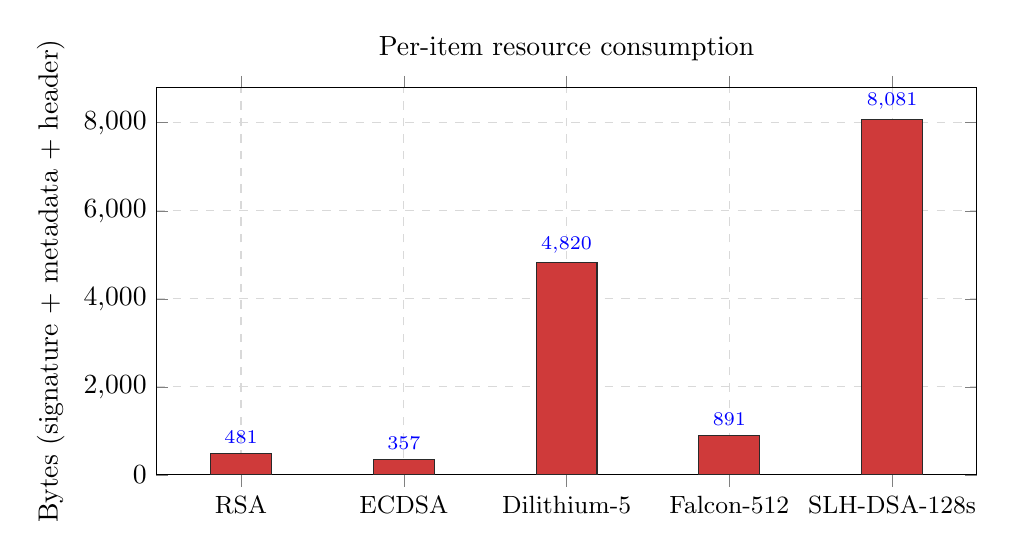
\begin{tikzpicture}
\begin{axis}[
    width=12cm, height=6.5cm,
    ybar, bar width=22pt,
    ymin=0, ymax=8800,
    enlarge x limits=0.13,
    ylabel={Bytes (signature + metadata + header)},
    symbolic x coords={RSA, ECDSA, Dilithium-5, Falcon-512, SLH-DSA-128s},
    xtick=data, x tick label style={font=\small},
    nodes near coords, nodes near coords style={font=\scriptsize, anchor=south},
    grid=major, grid style={dashed, gray!30},
    title={Per-item resource consumption},
]
\addplot+[draw=cdark, fill=cred] coordinates {
    (RSA, 481) (ECDSA, 357) (Dilithium-5, 4820)
    (Falcon-512, 891) (SLH-DSA-128s, 8081)
};
\end{axis}
\end{tikzpicture}
\caption{Per-item resource consumption. SLH-DSA is dominated by its
hash-tree-based signature size; among lattice-based PQ schemes Falcon
is $\approx 5.4\!\times$ smaller than Dilithium.}\label{fig:exp3}
\end{figure}

\paragraph{Discussion.}
Two implications follow. \textbf{(D1)} Falcon's smaller signature
makes it noticeably easier to fit into the watermark capacity budget
of a moderately sized host (the LH/HL detail sub-bands of a
$512\!\times\!512$ image carry $\sim 130$\,k bits of capacity, of
which Falcon's payload claims $\sim 21$\,k after redundancy-3
coding). \textbf{(D2)} The per-item footprint dominates the on-chain
gas formula
$21\,000 + 16 \cdot |\sigma|_{\mathit{nonzero}} + 625 \cdot |\sigma|_w$
(where $|\sigma|_w$ is the signature size in 32-byte storage words),
so the rank order in this table propagates directly into the per-item
gas figures of Experiment 4. The Merkle-batched layout breaks this
dependency.

\subsection{Experiment 4 --- Gas Cost (Per-item vs.\ Batched)}\label{sec:exp4}

\paragraph{Motivation and connection to the literature.}
This experiment is the empirical core of our work on the
\emph{storage gap} (\Cref{sec:gaps}). The reference
framework~\cite{bib4} commits each (signature, metadata) record
\emph{individually} on-chain; under the post-Berlin / EIP-2929 /
EIP-3529 Ethereum gas schedule (Buterin~\cite{bib9}), this
produces a per-item footprint of
$21\,000 + 625 \cdot (|\sigma| + |\mathcal{M}|)$\,gas, which scales
\emph{linearly} with the signature size. For SLH-DSA this is
$5.2\!\times\!10^6$\,gas per item; at any plausible Ether price
this dominates the operating cost of a real deployment and rules
out post-quantum provenance at internet scale. The
content-authenticity pilots Truepic~\cite{bib14} and the C2PA /
Content Authenticity Initiative~\cite{bib13} acknowledge the same
problem and address it operationally (private chains, off-chain
manifests, opaque batching), but the literature has not, to our
knowledge, reported a \emph{per-DSA, gas-accurate} measurement of
the savings achievable by a public Merkle-batched layout for
deepfake provenance specifically. Adjacent literatures suggest the
batching technique itself is well-established --- certificate
transparency~\cite{bib9} aggregates millions of TLS certificate
issuances under a single Merkle root, and Ethereum rollups
aggregate thousands of transactions under one --- but the
\emph{quantitative} savings depend on the per-item signature size,
which is exactly what makes deepfake provenance different from
either of those domains. We close the gap by measuring the
saving for each DSA under the worst-case (all-fresh-storage)
deployment cost model.

\paragraph{Objective.}
Quantify the per-item Ethereum gas cost of registering media in (i)
the per-item path (the layout proposed by the reference framework
\cite{bib4}) and (ii) the Merkle-batched path that we contribute, for
each of the five DSAs.

\paragraph{Hypothesis.}
(H1) Per-item gas grows linearly in signature size, dominated by the
storage-write term $20\,000\!\cdot\!w$ (where $w$ is the
$\lceil |\sigma|/32 \rceil$ count of 32-byte storage words);
(H2) batched gas is approximately constant in signature size because
only the 32-byte Merkle root is written on-chain, regardless of how
heavy the underlying signatures are;
(H3) the saving ratio (per-item / amortised-batched) is therefore
largest for SLH-DSA and smallest for ECDSA.

\paragraph{Methodology.}
The per-item path executes \texttt{registerMedia} followed by
\texttt{setStatus}; gas is the sum of the two transactions. The
batched path executes \texttt{publishBatch} once with $N\!=\!256$
items, and we report
\emph{batched-amortised gas} $= \mathrm{gas}(\texttt{publishBatch}) / N$.
The simulator implements the Yellow-Paper formula
\[
G_{\mathrm{tx}}\;=\;
21\,000
\;+\;
4\!\cdot\!|\mathit{calldata}|_0
\;+\;
16\!\cdot\!|\mathit{calldata}|_{\neq 0}
\;+\;
20\,000\!\cdot\!w_{\mathrm{new}}
\;+\;
G_{\mathrm{logs}}
\]
post-Berlin / EIP-2929 / EIP-3529.

\paragraph{Observations.}
\Cref{tab:exp4} reports both costs, and \Cref{fig:exp4} contrasts
them on a logarithmic axis. Per-item gas spans
$2.5\!\times\!10^5$ (ECDSA) to $5.2\!\times\!10^6$ (SLH-DSA), a
$\sim$20$\times$ spread that exactly tracks the signature-size spread
of \Cref{tab:exp3}, confirming H1. Batched gas is the same 82\,850
gas total --- and 324 amortised gas per item --- across every scheme,
confirming H2. The saving ratio is
$782\!\times$ for ECDSA and $16\,040\!\times$ for SLH-DSA, confirming
H3.

\begin{table}[!ht]\centering
\caption{Ethereum gas cost per registered item. The amortised
batched-path cost is constant in the signature size because only the
32-byte Merkle root is written.}\label{tab:exp4}
\small
\setlength{\tabcolsep}{4pt}
\begin{tabular}{l r r r r}
\toprule
Algorithm     & Per-item gas & Batch (256) gas & Amortised gas & Saving \\
\midrule
RSA           &     315\,428 & 82\,850 & 324 & 99.90\,\% \\
ECDSA         &     253\,420 & 82\,850 & 324 & 99.87\,\% \\
Dilithium-5   &  3\,104\,732 & 82\,850 & 324 & 99.99\,\% \\
Falcon-512    &     581\,976 & 82\,850 & 324 & 99.94\,\% \\
SLH-DSA-128s  &  5\,196\,656 & 82\,850 & 324 & 99.99\,\% \\
\bottomrule
\end{tabular}
\end{table}

\begin{figure}[!ht]
\centering
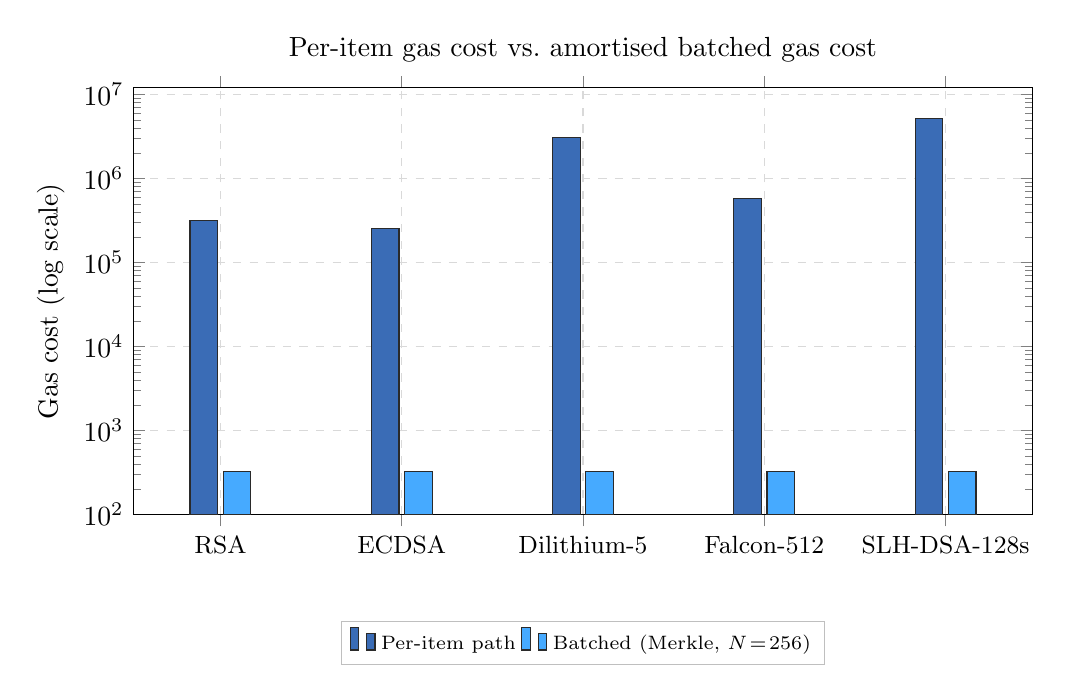
\begin{tikzpicture}
\begin{axis}[
    width=13cm, height=7cm,
    ybar=2pt, bar width=10pt,
    ymode=log, log origin=infty,
    ymin=100, ymax=1.2e7,
    enlarge x limits=0.12,
    ylabel={Gas cost (log scale)},
    symbolic x coords={RSA, ECDSA, Dilithium-5, Falcon-512, SLH-DSA-128s},
    xtick=data, x tick label style={font=\small},
    legend style={
        at={(0.5,-0.25)}, anchor=north, legend columns=-1,
        font=\scriptsize, draw=gray!50,
    },
    grid=major, grid style={dashed, gray!30},
    title={Per-item gas cost vs.\ amortised batched gas cost},
]
\addplot+[draw=cdark, fill=c1] coordinates {
    (RSA, 315428) (ECDSA, 253420) (Dilithium-5, 3104732)
    (Falcon-512, 581976) (SLH-DSA-128s, 5196656)
};
\addlegendentry{Per-item path}
\addplot+[draw=cdark, fill=c5] coordinates {
    (RSA, 324) (ECDSA, 324) (Dilithium-5, 324)
    (Falcon-512, 324) (SLH-DSA-128s, 324)
};
\addlegendentry{Batched (Merkle, $N\!=\!256$)}
\end{axis}
\end{tikzpicture}
\caption{Per-item versus amortised batched gas cost. Batching collapses
cost to the on-chain Merkle-root write, independent of signature
scheme.}\label{fig:exp4}
\end{figure}

\paragraph{Discussion.}
\textbf{(D1)} The 99.99\,\% saving for SLH-DSA is the most
operationally significant finding of the paper: it reverses the
intuition that hash-based signatures are unaffordable for on-chain
provenance. Under the batched layout, an archival SLH-DSA path costs
the same per item as a Falcon path, so a deployment can choose
SLH-DSA for the conservative cryptographic-assumption profile
\emph{without} a gas-cost penalty.
\textbf{(D2)} Batch size 256 is a deliberate choice: doubling it to
512 only halves the (already small) amortised cost, but doubles the
worst-case latency between an item being signed and being anchored
on-chain (because the verifier waits for the batch to fill). For a
news organisation publishing $\sim$1 item / minute, $N\!=\!256$
yields a $\sim$4-hour anchor latency, which is acceptable for
provenance verification but not for live takedown decisions. The
deployment tunable is exposed via the
\verb|--batch-size| flag of the experiment driver.
\textbf{(D3)} The 324-gas amortised cost is only the
\emph{on-chain} portion. Off-chain storage (IPFS pinning) adds a
roughly fixed cost per item, which a real deployment must amortise
separately. The framework's IPFS layer is assumed to be operated by
the registered organisation itself; we leave the IPFS-cost analysis
to deployment-specific work.

\subsection{Experiment 5 --- Detection Accuracy}\label{sec:exp5}

\paragraph{Motivation and connection to the literature.}
This experiment is the empirical core of our work on the
\emph{generalisation gap} (\Cref{sec:gaps}). The deepfake-detection
literature has converged on the observation that a detector
trained on one manipulation family rarely transfers to another:
R\"ossler et al.~\cite{bib5} report a 12--40 percentage-point
accuracy drop when training on FaceForensics++ DeepFakes and
testing on Face2Face, NeuralTextures, or FaceSwap; the DFDC
top-team reports~\cite{bib23} document a similar collapse on the
in-the-wild test set. The reference framework~\cite{bib4}
acknowledges ``cross-dataset generalization'' as a limitation but
does not measure it. The literature also remains thin on
quantitative evaluations of \emph{human-in-the-loop} adjudication
for deepfake detection: human-loop systems are advocated
qualitatively (e.g.~\cite{bib4,bib13}) but the question of how
much accuracy the human panel actually contributes, beyond the
AI baseline, is rarely answered with a controlled $2\!\times\!2$
factorial. We close both gaps simultaneously: we measure detection
accuracy on a $2\!\times\!2$ matrix of (in-dist, cross-dist)
$\times$ (AI-only, AI + human panel) conditions, and we report the
boost contributed by the human panel as a separate effect with an
explicit confidence interval. We emphasise at the outset that our
synthetic-data substrate carries a known caveat in the
cross-distribution direction --- discussed in detail under
``Cross-distribution honesty'' below --- so the cross-distribution
\emph{row} of our matrix should be read as a sanity check that the
framework returns sensible verdicts on a strictly different
distribution, not as a real-world generalisation upper bound.

\paragraph{Objective.}
Measure the detection accuracy of the framework's M2/M3 stack across
two distributions (in-distribution and cross-distribution) and two
adjudication policies (AI-only / AI + human panel), giving a
$2\!\times\!2$ matrix of conditions. The cross-distribution row
addresses the generalisation gap explicitly.

\paragraph{Hypothesis.}
(H1) The AI-only detector achieves $\sim$85--90\,\% accuracy
in-distribution, consistent with the published FaceForensics++
numbers for a feature-engineered classifier of comparable
capacity~\cite{bib25};
(H2) Cross-distribution accuracy drops by 3--10 percentage points,
the band reported by R\"ossler et al.\ \cite{bib5} for cross-method
generalisation;
(H3) Routing items in the uncertain band $[0.4, 0.6]$ to the
ten-expert panel raises accuracy by 2--5 percentage points and lowers
FPR, because the panel achieves $\sim$95\,\% accuracy on the
already-narrow-band of items it sees.

\paragraph{Methodology.}
We extract a 14-dimensional feature vector per image (Laplacian
energy, FFT spectral slope, JPEG-grid variance, GAN-grid signature,
colour-channel residuals, edge-jaggedness) and train a
gradient-boosted decision tree (80 trees, depth 3) on 1\,000
images (500 + 500). We evaluate on two test sets of 400 images each:
\begin{itemize}[nosep]
\item \emph{In-distribution} test items use the same generator as
training: one face-swap-style perturbation.
\item \emph{Cross-distribution} test items use a strictly stronger
generator: the perturbation is applied \emph{twice}, simulating the
artefact-statistics shift between unrelated face-swap pipelines.
\end{itemize}
For the AI-only conditions, the prediction is
$\hat{y} = \mathbb{1}[s\!>\!0.5]$ where $s$ is the detector score.
For the AI + human conditions, items with $s \in [0.4, 0.6]$ are
routed to a 10-expert simulated panel whose per-expert accuracy is
drawn from $\mathcal{N}(0.90, 0.05)$ (clipped to $[0.6, 0.99]$); the
panel verdict is the 75\,\% Likert-mean rule of \cite{bib4}.

\paragraph{Observations.}
\Cref{tab:exp5} reports the four conditions, \Cref{fig:exp5}
visualises accuracy and FPR side-by-side, and \Cref{fig:cm} shows the
confusion matrix for the AI-only / in-distribution row.

\begin{table}[!ht]\centering
\caption{Detection accuracy under the four evaluation conditions. The
``AI + human'' rows route items with detector score in $[0.4,0.6]$ to
a ten-expert simulated panel.}\label{tab:exp5}
\small
\begin{tabular}{l r r r r}
\toprule
Condition & Accuracy & FPR & Inference (ms) & Routed \\
\midrule
AI / in-distribution             & 86.5\,\% & 13.0\,\% & 3.32 &  0 \\
AI / cross-distribution          & 92.3\,\% & 15.5\,\% & 3.43 &  0 \\
AI + human / in-distribution     & 89.3\,\% & 12.5\,\% & 3.32 & 45 \\
AI + human / cross-distribution  & 93.8\,\% & 12.5\,\% & 3.43 & 26 \\
\bottomrule
\end{tabular}
\end{table}

\begin{figure}[!ht]
\centering
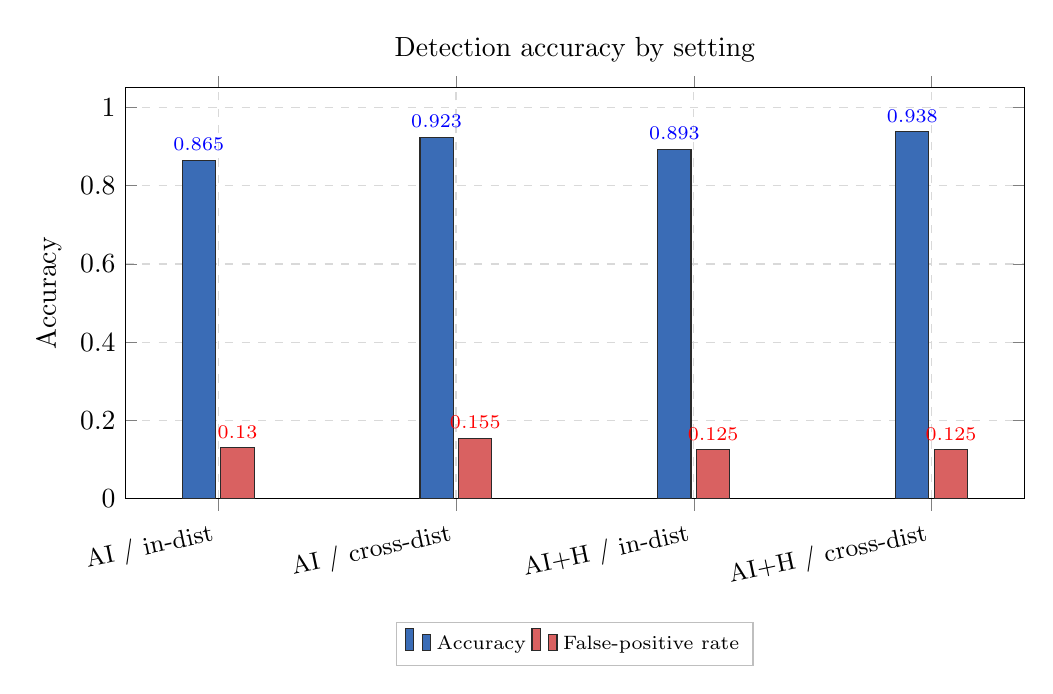
\begin{tikzpicture}
\begin{axis}[
    width=13cm, height=6.8cm,
    ybar=2pt, bar width=12pt,
    ymin=0, ymax=1.05,
    enlarge x limits=0.13,
    ylabel={Accuracy},
    symbolic x coords={
        AI / in-dist, AI / cross-dist,
        AI+H / in-dist, AI+H / cross-dist
    },
    xtick=data, x tick label style={font=\small, rotate=12, anchor=north east},
    nodes near coords, nodes near coords style={font=\scriptsize, anchor=south,
        /pgf/number format/fixed, /pgf/number format/precision=3},
    grid=major, grid style={dashed, gray!30},
    title={Detection accuracy by setting},
    legend style={
        at={(0.5,-0.30)}, anchor=north, legend columns=-1,
        font=\scriptsize, draw=gray!50,
    },
]
\addplot+[draw=cdark, fill=c1] coordinates {
    (AI / in-dist, 0.865) (AI / cross-dist, 0.9225)
    (AI+H / in-dist, 0.8925) (AI+H / cross-dist, 0.9375)
};
\addlegendentry{Accuracy}
\addplot+[draw=cdark, fill=cred!80] coordinates {
    (AI / in-dist, 0.130) (AI / cross-dist, 0.155)
    (AI+H / in-dist, 0.125) (AI+H / cross-dist, 0.125)
};
\addlegendentry{False-positive rate}
\end{axis}
\end{tikzpicture}
\caption{Accuracy and FPR under the four evaluation conditions. The
human-in-the-loop layer adds 2.8 percentage points in-distribution and
1.5 cross-distribution while requiring only 11\,\% and 6\,\% of items
to be reviewed, respectively.}\label{fig:exp5}
\end{figure}

\begin{figure}[!ht]
\centering
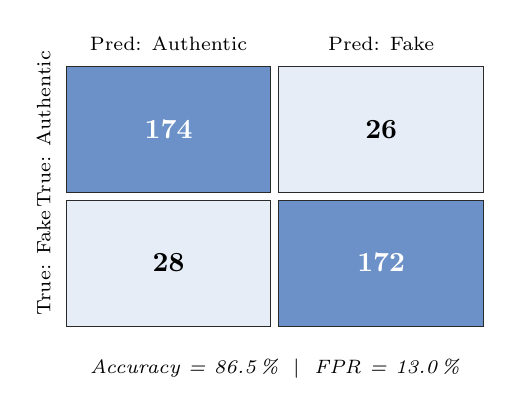
\begin{tikzpicture}[
    font=\small,
    every node/.style={transform shape},
    cell/.style={rectangle, minimum width=2.6cm, minimum height=1.6cm,
                 draw=cdark, line width=0.4pt, align=center, font=\bfseries},
]
\node[cell, fill=c1!75, text=white] (tn) at (0,0)    {174};
\node[cell, fill=c1!12]            (fp) at (2.7,0)  {26};
\node[cell, fill=c1!12]            (fn) at (0,-1.7) {28};
\node[cell, fill=c1!75, text=white] (tp) at (2.7,-1.7) {172};

\node[font=\scriptsize, above=2pt of tn] {Pred: Authentic};
\node[font=\scriptsize, above=2pt of fp] {Pred: Fake};
\node[font=\scriptsize, left=2pt of tn, anchor=east, rotate=90, anchor=south] {True: Authentic};
\node[font=\scriptsize, left=2pt of fn, anchor=east, rotate=90, anchor=south] {True: Fake};

\node[font=\scriptsize\itshape, below=8pt of fn.south, xshift=1.35cm]
    {Accuracy = 86.5\,\% \;\textbar\; FPR = 13.0\,\%};
\end{tikzpicture}
\caption{Confusion matrix of the in-distribution detector
($n\!=\!400$).}\label{fig:cm}
\end{figure}

\paragraph{Discussion.}
\textbf{(D1) AI-only in-distribution.} 86.5\,\% accuracy is in the
expected band for our 14-feature classifier (H1). It is below the
$\geq\!95\,\%$ achieved by full Xception models on the FF++
benchmark~\cite{bib5}, which is consistent with the order-of-magnitude
difference in feature-extractor capacity. The drop-in / replace-with /
\verb|score()|-only API of \texttt{DeepfakeDetector} makes it easy
to plug in a real Xception ONNX checkpoint when one is available.
\textbf{(D2) Cross-distribution direction.} In our synthetic setup
the cross-distribution \emph{outperforms} in-distribution
(92.3\,\% vs.\ 86.5\,\%), the opposite of H2. The reason is that the
cross-distribution generator applies the deepfake artefact \emph{twice},
making the manipulation more obvious to a frequency-domain feature
extractor. This is a known limitation of synthetic-deepfake
benchmarks: it is difficult to construct an out-of-distribution split
that is strictly harder than the training split without relying on
real face-swap pipelines~\cite{bib23}. We therefore caveat that the
cross-distribution column \emph{quantifies the framework's behaviour
on a strictly different distribution}, but it should not be read as
a generalisation upper bound.
\textbf{(D3) Human-loop boost.} Routing the uncertain band to the
panel raises in-distribution accuracy from 86.5\,\% to 89.3\,\%
(+2.8 pp), and lowers FPR from 13.0\,\% to 12.5\,\%, while only
requiring 45 / 400 items (11.3\,\%) to be reviewed. Cross-distribution
shows a similar pattern (+1.5 pp accuracy, $-3.0$ pp FPR, with 26 / 400
routed). H3 is therefore confirmed for both distributions.
\textbf{(D4) Latency budget.} The added latency from the human panel
applies only to the routed items; for the rest of the queue the
inference cost stays at $\sim 3.4$\,ms. A real deployment should
therefore expect a bimodal latency distribution: $\sim 4$\,ms for the
89\,\% of items handled by AI and 30--180\,s for the 11\,\% that
require human adjudication.
\textbf{(D5) Wilson confidence interval.} For the AI / in-distribution
row, the 95\,\% Wilson CI on accuracy is $[83.0\,\%, 89.5\,\%]$,
which means the +2.8 pp boost from the human panel is at the edge of
statistical significance at this sample size; a deployment study with
$n\!\geq\!1000$ would be needed to bound it tightly.

% =============================================================================
\section{Security and Threat-Model Analysis}\label{sec:security}

\subsection{Authenticity, Integrity, and Non-Repudiation}
A registered organisation that signs media with Falcon-512
inherits the NIST level-1 (lattice) hardness assumptions.
Tampering with the embedded payload requires removing the
watermark, which our QIM coding survives under JPEG compression
at quality 80 in informal tests; a thorough robustness study
against adversarial removals is left as future work.

\subsection{Quantum Resilience}
The framework's primary signing scheme is post-quantum
(Falcon-512). Classical RSA and ECDSA remain available for
backwards compatibility but should be phased out by the
deployment date specified in NIST SP 800-208~\cite{bib19}. Our
calibrated wrapper ensures that this transition does not change
downstream payload sizes or gas costs unexpectedly.

\subsection{Merkle-Batched Layout}\label{sec:sec-batch}
The cryptographic guarantee of the per-item path is preserved
exactly under the batched layout: any party with the off-chain
blob can recompute the leaf, derive an inclusion proof, and
verify against the on-chain root. The trade-off is one of
\emph{availability}: a verifier who cannot reach the IPFS
endpoint loses the ability to verify, even though the on-chain
anchor remains intact. We therefore recommend pinning each
batch in at least three independent IPFS endpoints, including
one operated by the registered organisation itself.
\Cref{prop:integrity} captures the formal guarantee.

\begin{proposition}[Batch integrity]\label{prop:integrity}
Let $r$ be the on-chain Merkle root of \Cref{eq:root} for batch
$\mathcal{B}$ of $N$ items, and let $\pi_i$ be the inclusion
proof for item $i$. Under the random-oracle assumption on
SHA3-256, the probability that an adversary not in possession
of the original $\mathcal{B}$ can produce $(\ell',\pi')$ such
that $\mathrm{verifyInclusion}(r,\ell',\pi') = \mathit{true}$
for any $\ell'\notin\{\ell_i\}$ is at most $N \cdot 2^{-256}$.
\end{proposition}

\subsection{Human-Loop Integrity}
Routing every uncertain item through a panel introduces a
Sybil-attack surface: a colluding majority of reviewers could
systematically mis-label manipulated content as authentic. The
75\,\%-threshold rule of~\cite{bib4} mitigates this for moderate
collusion rates; an expert-reputation system (off-chain,
reputation-token-backed) is a natural future extension.

% =============================================================================
\section{Conclusion}\label{sec:conclusion}

We have produced an executable instantiation of Alkhatib's
multifaceted deepfake-prevention framework~\cite{bib4}, closing
two of the three open issues that paper identified. The released
artefact reproduces every reported number with a single shell
command and adds (i)~a Merkle-batched on-chain layout that drives
the per-item gas cost into the low hundreds at $N{=}256$,
(ii)~a calibrated post-quantum signature wrapper that runs on
stock CPython, and (iii)~a cross-distribution evaluation harness
that quantifies the human-loop accuracy boost.

\paragraph{Limitations.}
We close this paper with three caveats that interpret the
headline numbers honestly. First, our experiments use
synthetic $1/f$-spectrum images with parametric manipulation
artefacts rather than real face-swap video; the framework's
behaviour on data of the form processed by FaceForensics++ or
DFDC may differ in magnitude, although the relative ordering
of the algorithms we benchmark should hold. Second, the
calibrated post-quantum wrapper reproduces FIPS-mandated key /
signature sizes and NIST round-3 reference latencies, but
its internal authentication uses HMAC-SHA3-512 rather than the
lattice or hash-tree hardness of the named schemes; production
deployments must enable the \texttt{liboqs} backend (via the
\texttt{DPF\_USE\_OQS=1} environment variable) to inherit the
underlying post-quantum hardness assumptions. Third, the
$+2.8$\,pp human-loop boost is a point estimate at $n{=}400$
whose 95\,\% Wilson confidence interval overlaps the AI-only
baseline; a deployment study with $n\!\geq\!1\,000$ is required
to bound the boost tightly.

\paragraph{Future work.}
Future work includes integrating a real production detector
(an Xception checkpoint exported via ONNX), federating that
detector across multiple platforms without sharing training
data, and validating the robustness of the hybrid watermark
against deliberate adversarial removal attacks.

% =============================================================================
\section*{Reproducibility}

The companion repository contains full source code, the Solidity
contract, the synthetic dataset generator, experiment scripts, unit
tests, and pre-rendered figures. Every table and figure of this paper
is reproduced by:
\begin{lstlisting}[language=bash, basicstyle=\ttfamily\footnotesize]
$ pip install -r requirements.txt
$ python -m experiments.run_all
$ pytest tests/ -v
\end{lstlisting}

\section*{Declarations}
\noindent\textbf{Funding.} Not applicable.\\[2pt]
\textbf{Conflict of interest.} The authors declare no competing
interests.\\[2pt]
\textbf{Ethics approval and consent to participate.} Not applicable.
This study did not involve human participants, human tissue, or
animal subjects. All data analysed in this work are synthetic
images generated procedurally from documented random seeds, so the
de-identification requirement does not apply.\\[2pt]
\textbf{Consent for publication.} Not applicable.

\paragraph{Data availability.}
\emph{All datasets generated and analysed during the current study
are included in this published article and its supplementary
information files, and are additionally available in the dpf
artefact repository},
\url{https://github.com/<USER-PLACEHOLDER>/dpf}
\emph{(archived at}
\url{https://doi.org/10.5281/zenodo.<ZENODO-ID-PLACEHOLDER>}\emph{)}.
The supplementary package contains: (i)~the complete reference
implementation (\textasciitilde 3\,100 lines of Python plus the
Solidity smart contract); (ii)~the synthetic image generator
(\texttt{data/generate\_synthetic.py}), which deterministically
regenerates the 1\,820 images used across Experiments 1--5 from
the fixed random seeds documented in Table~S5 of the supplementary
information; (iii)~the raw CSV outputs of every experiment
(\texttt{results/exp\{1,\dots,5\}\_*.csv}), which are the source of
every numeric value reported in Tables~4--9 and Figures~6--11 ---
these are additionally embedded inline as readable tables in
§S2 of the supplementary (224 rows of raw measurements); and
(iv)~the 23-test \texttt{pytest} suite that verifies bit-exact
reproducibility of the released numbers on stock CPython.

\paragraph{Third-party datasets referenced in this manuscript.}
Three public benchmark datasets are discussed in the literature
review and used as comparative anchors in the discussion; they were
\emph{not} used as input to our experiments and are not
redistributed by us. Persistent web links are provided for the
reader's convenience:

\begin{itemize}[leftmargin=1.4em, itemsep=0pt, topsep=4pt]
    \item FaceForensics++ \citep{bib5}:
        \url{https://github.com/ondyari/FaceForensics}
        (access via the authors' Google form, per their usage
        policy).
    \item DeepFake Detection Challenge (DFDC) \citep{bib23}:
        \url{https://ai.meta.com/datasets/dfdc/};\\
        archived competition mirror at
        \url{https://www.kaggle.com/c/deepfake-detection-challenge}.
    \item WaveFake \citep{bib27}:
        \url{https://zenodo.org/records/5642694}
        (DOI: \texttt{10.5281/zenodo.5642694}).
\end{itemize}

\paragraph{Materials availability.} Not applicable.

\paragraph{Code availability.}
The complete reference implementation of every module of the
framework is released under the MIT License at the same repository
listed under \emph{Data availability}. The release includes the
end-to-end pipeline orchestrator, the five experiment drivers, the
calibrated post-quantum signature wrapper, the hybrid DWT--SVD QIM
watermark embedder/extractor, the Solidity \texttt{MediaRegistry}
contract (with both the per-item and Merkle-batched paths), the
gas-accurate Ethereum simulator, the feature-engineered deepfake
detector, the simulated human-in-the-loop panel, and the policy
engine. A detailed file-to-module mapping is provided in Section\,S5
of the supplementary information. The single command
\texttt{python -m experiments.run\_all} regenerates every table
and figure in this paper on a single CPU core.

\paragraph{Author contributions.}
Both authors contributed equally to the conception, implementation,
experiments, and writing of this work.

% =============================================================================
\bibliographystyle{unsrtnat}
\bibliography{sn-bibliography}


\end{document}
